\documentclass[12pt,a4paper]{book}
\usepackage{lmodern}
\usepackage{amssymb,amsmath}
\usepackage{ifxetex,ifluatex}
\usepackage{fixltx2e} % provides \textsubscript
\ifnum 0\ifxetex 1\fi\ifluatex 1\fi=0 % if pdftex
  \usepackage[T1]{fontenc}
  \usepackage[utf8]{inputenc}
\else % if luatex or xelatex
  \ifxetex
    \usepackage{mathspec}
  \else
    \usepackage{fontspec}
  \fi
  \defaultfontfeatures{Ligatures=TeX,Scale=MatchLowercase}
\fi
% use upquote if available, for straight quotes in verbatim environments
\IfFileExists{upquote.sty}{\usepackage{upquote}}{}
% use microtype if available
\IfFileExists{microtype.sty}{%
\usepackage{microtype}
\UseMicrotypeSet[protrusion]{basicmath} % disable protrusion for tt fonts
}{}
\usepackage[margin=1in]{geometry}
\usepackage{hyperref}
\PassOptionsToPackage{usenames,dvipsnames}{color} % color is loaded by hyperref
\hypersetup{unicode=true,
            colorlinks=true,
            linkcolor=Maroon,
            citecolor=Blue,
            urlcolor=blue,
            breaklinks=true}
\urlstyle{same}  % don't use monospace font for urls
\usepackage{natbib}
\bibliographystyle{plainnat}
\usepackage{color}
\usepackage{fancyvrb}
\newcommand{\VerbBar}{|}
\newcommand{\VERB}{\Verb[commandchars=\\\{\}]}
\DefineVerbatimEnvironment{Highlighting}{Verbatim}{commandchars=\\\{\}}
% Add ',fontsize=\small' for more characters per line
\usepackage{framed}
\definecolor{shadecolor}{RGB}{248,248,248}
\newenvironment{Shaded}{\begin{snugshade}}{\end{snugshade}}
\newcommand{\KeywordTok}[1]{\textcolor[rgb]{0.13,0.29,0.53}{\textbf{#1}}}
\newcommand{\DataTypeTok}[1]{\textcolor[rgb]{0.13,0.29,0.53}{#1}}
\newcommand{\DecValTok}[1]{\textcolor[rgb]{0.00,0.00,0.81}{#1}}
\newcommand{\BaseNTok}[1]{\textcolor[rgb]{0.00,0.00,0.81}{#1}}
\newcommand{\FloatTok}[1]{\textcolor[rgb]{0.00,0.00,0.81}{#1}}
\newcommand{\ConstantTok}[1]{\textcolor[rgb]{0.00,0.00,0.00}{#1}}
\newcommand{\CharTok}[1]{\textcolor[rgb]{0.31,0.60,0.02}{#1}}
\newcommand{\SpecialCharTok}[1]{\textcolor[rgb]{0.00,0.00,0.00}{#1}}
\newcommand{\StringTok}[1]{\textcolor[rgb]{0.31,0.60,0.02}{#1}}
\newcommand{\VerbatimStringTok}[1]{\textcolor[rgb]{0.31,0.60,0.02}{#1}}
\newcommand{\SpecialStringTok}[1]{\textcolor[rgb]{0.31,0.60,0.02}{#1}}
\newcommand{\ImportTok}[1]{#1}
\newcommand{\CommentTok}[1]{\textcolor[rgb]{0.56,0.35,0.01}{\textit{#1}}}
\newcommand{\DocumentationTok}[1]{\textcolor[rgb]{0.56,0.35,0.01}{\textbf{\textit{#1}}}}
\newcommand{\AnnotationTok}[1]{\textcolor[rgb]{0.56,0.35,0.01}{\textbf{\textit{#1}}}}
\newcommand{\CommentVarTok}[1]{\textcolor[rgb]{0.56,0.35,0.01}{\textbf{\textit{#1}}}}
\newcommand{\OtherTok}[1]{\textcolor[rgb]{0.56,0.35,0.01}{#1}}
\newcommand{\FunctionTok}[1]{\textcolor[rgb]{0.00,0.00,0.00}{#1}}
\newcommand{\VariableTok}[1]{\textcolor[rgb]{0.00,0.00,0.00}{#1}}
\newcommand{\ControlFlowTok}[1]{\textcolor[rgb]{0.13,0.29,0.53}{\textbf{#1}}}
\newcommand{\OperatorTok}[1]{\textcolor[rgb]{0.81,0.36,0.00}{\textbf{#1}}}
\newcommand{\BuiltInTok}[1]{#1}
\newcommand{\ExtensionTok}[1]{#1}
\newcommand{\PreprocessorTok}[1]{\textcolor[rgb]{0.56,0.35,0.01}{\textit{#1}}}
\newcommand{\AttributeTok}[1]{\textcolor[rgb]{0.77,0.63,0.00}{#1}}
\newcommand{\RegionMarkerTok}[1]{#1}
\newcommand{\InformationTok}[1]{\textcolor[rgb]{0.56,0.35,0.01}{\textbf{\textit{#1}}}}
\newcommand{\WarningTok}[1]{\textcolor[rgb]{0.56,0.35,0.01}{\textbf{\textit{#1}}}}
\newcommand{\AlertTok}[1]{\textcolor[rgb]{0.94,0.16,0.16}{#1}}
\newcommand{\ErrorTok}[1]{\textcolor[rgb]{0.64,0.00,0.00}{\textbf{#1}}}
\newcommand{\NormalTok}[1]{#1}
\usepackage{longtable,booktabs}
\usepackage{graphicx,grffile}
\makeatletter
\def\maxwidth{\ifdim\Gin@nat@width>\linewidth\linewidth\else\Gin@nat@width\fi}
\def\maxheight{\ifdim\Gin@nat@height>\textheight\textheight\else\Gin@nat@height\fi}
\makeatother
% Scale images if necessary, so that they will not overflow the page
% margins by default, and it is still possible to overwrite the defaults
% using explicit options in \includegraphics[width, height, ...]{}
\setkeys{Gin}{width=\maxwidth,height=\maxheight,keepaspectratio}
\IfFileExists{parskip.sty}{%
\usepackage{parskip}
}{% else
\setlength{\parindent}{0pt}
\setlength{\parskip}{6pt plus 2pt minus 1pt}
}
\setlength{\emergencystretch}{3em}  % prevent overfull lines
\providecommand{\tightlist}{%
  \setlength{\itemsep}{0pt}\setlength{\parskip}{0pt}}
\setcounter{secnumdepth}{5}
% Redefines (sub)paragraphs to behave more like sections
\ifx\paragraph\undefined\else
\let\oldparagraph\paragraph
\renewcommand{\paragraph}[1]{\oldparagraph{#1}\mbox{}}
\fi
\ifx\subparagraph\undefined\else
\let\oldsubparagraph\subparagraph
\renewcommand{\subparagraph}[1]{\oldsubparagraph{#1}\mbox{}}
\fi

%%% Use protect on footnotes to avoid problems with footnotes in titles
\let\rmarkdownfootnote\footnote%
\def\footnote{\protect\rmarkdownfootnote}

%%% Change title format to be more compact
\usepackage{titling}

% Create subtitle command for use in maketitle
\newcommand{\subtitle}[1]{
  \posttitle{
    \begin{center}\large#1\end{center}
    }
}

\setlength{\droptitle}{-2em}
  \title{\textbf{\LARGE R을 이용한 자료처리 및 시각화}}
  \pretitle{\vspace{\droptitle}\centering\huge}
  \posttitle{\par}
\subtitle{\textbf{\Large 기본 환경 설정부터 재현가능한 연구 방법 입문}\vspace{2cm}\linebreak 한국한의학연구원
한의기반연구부\linebreak Korea Institute of Oriental Medicine, KM
Fundamental Research Division \vspace{2cm}}
  \author{\textbf{\Large 구본초, Ph.D. in Statistics}}
  \preauthor{\centering\large\emph}
  \postauthor{\par}
  \predate{\centering\large\emph}
  \postdate{\par}
  \date{2017-11-23}

\usepackage{kotex}
\usepackage{xspace}
\usepackage{placeins}
\usepackage{enumerate}
\usepackage{float}
\usepackage{setspace}\doublespacing
\usepackage{relsize}
\usepackage{bigints}
\usepackage{bm}
\usepackage{lipsum}
\usepackage{booktabs}
\usepackage{dcolumn}
\usepackage{array}
\usepackage[font=small,labelfont=bf]{caption}
\usepackage{gensymb}
\usepackage{makecell}
\usepackage{multirow}
\usepackage{natbib}
\usepackage{threeparttable}
\usepackage{rotating}
\usepackage[table]{xcolor}
\usepackage{graphicx,grffile}
\usepackage{tikz}
\usetikzlibrary{shadows}

\newcommand*\keystroke[1]{%
  \tikz[baseline=(key.base)]
    \node[%
      draw,
      fill=white,
      drop shadow={shadow xshift=0.25ex,shadow yshift=-0.25ex,fill=black,opacity=0.75},
      rectangle,
      rounded corners=2pt,
      inner sep=1pt,
      line width=0.5pt,
      font=\scriptsize\sffamily
    ](key) {#1\strut}
  ;
}
\newcommand{\latex}{\LaTeX\xspace}

\renewcommand\theadalign{cb}
\renewcommand\theadfont{\bfseries}
\renewcommand\theadgape{\Gape[4pt]}
\renewcommand\cellgape{\Gape[4pt]}
\DeclareMathAlphabet{\mathpzc}{OT1}{pzc}{m}{it}

\renewcommand\theadalign{cb}
\renewcommand\theadfont{\bfseries}
\renewcommand\theadgape{\Gape[4pt]}
\renewcommand\cellgape{\Gape[4pt]}

\newcolumntype{L}[1]{>{\raggedright\let\newline\\
\arraybackslash\hspace{0pt}}m{#1}}
\newcolumntype{C}[1]{>{\centering\let\newline\\
\arraybackslash\hspace{0pt}}m{#1}}
\newcolumntype{R}[1]{>{\raggedleft\let\newline\\
\arraybackslash\hspace{0pt}}m{#1}}
\newcolumntype{P}[1]{>{\raggedright\tabularxbackslash}p{#1}}
\newcommand{\specialcell}[2][c]{%
  \begin{tabular}[#1]{@{}c@{}}#2\end{tabular}}
\newcommand{\specialcelll}[2][l]{%
  \begin{tabular}[#1]{@{}l@{}}#2\end{tabular}}


\captionsetup[table]{aboveskip=0pt}
\captionsetup[table]{belowskip=10pt}

\pagestyle{plain}
% \linespread{1.5}

\usepackage{amsthm}
\newtheorem{theorem}{Theorem}[chapter]
\newtheorem{lemma}{Lemma}[chapter]
\theoremstyle{definition}
\newtheorem{definition}{Definition}[chapter]
\newtheorem{corollary}{Corollary}[chapter]
\newtheorem{proposition}{Proposition}[chapter]
\theoremstyle{definition}
\newtheorem{example}{Example}[chapter]
\theoremstyle{definition}
\newtheorem{exercise}{Exercise}[chapter]
\theoremstyle{remark}
\newtheorem*{remark}{Remark}
\newtheorem*{solution}{Solution}
\begin{document}
\maketitle

{
\hypersetup{linkcolor=black}
\setcounter{tocdepth}{1}
\tableofcontents
}
\chapter{R을 사용하기 위한 환경 설정}\label{r----}

\section{Overview}\label{overview}

\subsection{What is R?}\label{what-is-r}

\begin{itemize}
\item
  R 언어: 통계 및 자료 시각화를 지원하는 언어 및 환경
\item
  1980년 AT\&T 연구소의 John Chambers가 개발한 S 언어를 기반으로 1995년
  뉴질랜드 Auckland Univ.의 Robert Gentleman \& Ross Ihaka 개발이 그
  기원임
\item
  GNU 기반 오픈소스
\end{itemize}

\subsection{Why R?}\label{why-r}

\begin{enumerate}
\def\labelenumi{\arabic{enumi}.}
\tightlist
\item
  장점

  \begin{itemize}
  \tightlist
  \item
    \textbf{Free software}
  \item
    주요 운영체제(Unix, Windows, Macintosh)에서 사용 가능
  \item
    현존하는 거의 대부분의 통계 방법론들이 package로 구현
  \item
    강력한 그래픽 기능
  \item
    빠른 update 및 연산속도(?)
  \item
    방대한 community 및 R package에 공개 및 공유된 자료
  \end{itemize}
\item
  Do we have to learn R language?

  \begin{itemize}
  \tightlist
  \item
    물론 꼭 배울 필요는 없다!! (요리를 하는데 꼭 좋은 칼이 필요
    없듯이\ldots{})
  \item
    다양한 통계 소프트웨어 및 분석 언어(SPSS, SAS, WEKA, MATLAB, PYTHON,
    \ldots{}) 존재
  \item
    프로그래밍에 익숙하지 않은 사용자들의 접근성이 떨어짐
  \item
    하지만 배워두면 좋은 이유

    \begin{itemize}
    \tightlist
    \item
      통계분석과 보고서 작성을 위한 최적 환경

      \begin{itemize}
      \tightlist
      \item
        R + Rstudio + Rmarkdown을 통해 분석에서부터 보고서 작성까지
        한번에 가능
      \end{itemize}
    \item
      SPSS, SAS에 비해 확장성이 높기 때문에 다양한 문제에 적용 가능
    \item
      방대한 양의 메뉴얼 및 서적들
    \item
      그리고 이 모든 것을 거의 대부분 무료 사용 가능
    \end{itemize}
  \end{itemize}
\end{enumerate}

\begin{quote}
\colorbox{gray!10}{\begin{minipage}{15cm}
\textbf{Tips}
  \begin{itemize}
    \item R에서 구현한 모든 package들은 CRAN (The Comprehensive R Archive Network, http://cran.r-project.org/web/view)에서 살펴볼 수 있음
    \item R과 관련한 대부분의 문제는 Google 검색과 스텍 오버플로우(http://stackoverflow.com)에서 해결할 수 있음
    \item 해당 문서는 서민구 선생님의 ``R을 이용한 데이터 처리 \& 실무'' \citep{Seo-2014} 와 고석범 선생님의 ``R과 Knitr을 활용한 데이터 연동형 문서 만들기'' \citep{Ko-2014} 의 내용을 주로 참조함. 
    \item: 해당 문서는 \texttt{RMarkdown} + \latex + \texttt{knitr}로 작성된 문서이며, 이를 위해 작성한 모든 소스 코드 및 자료는 https://github.com/Secondmoon-Kiom/CNUH-R-Lecture-2017 에서 확인할 수 있음. 
  \end{itemize}
\end{minipage}}
\end{quote}

\newpage

\section{R 설치하기(Windows 용)}\label{r-windows-}

R은 공개 소프트웨어로 \url{http://www.r-project.org/} 에서 다운로드 및
설치 가능

\begin{enumerate}
\def\labelenumi{\arabic{enumi}.}
\tightlist
\item
  웹브라우저(i.e.~explore, chrome, firefox 등)에서
  \url{http://www.r-project.org} 이동
\item
  좌측 R Logo 하단 Download 아래 `CRAN' 클릭
\end{enumerate}

\begin{figure}[H]
{
  \centering
  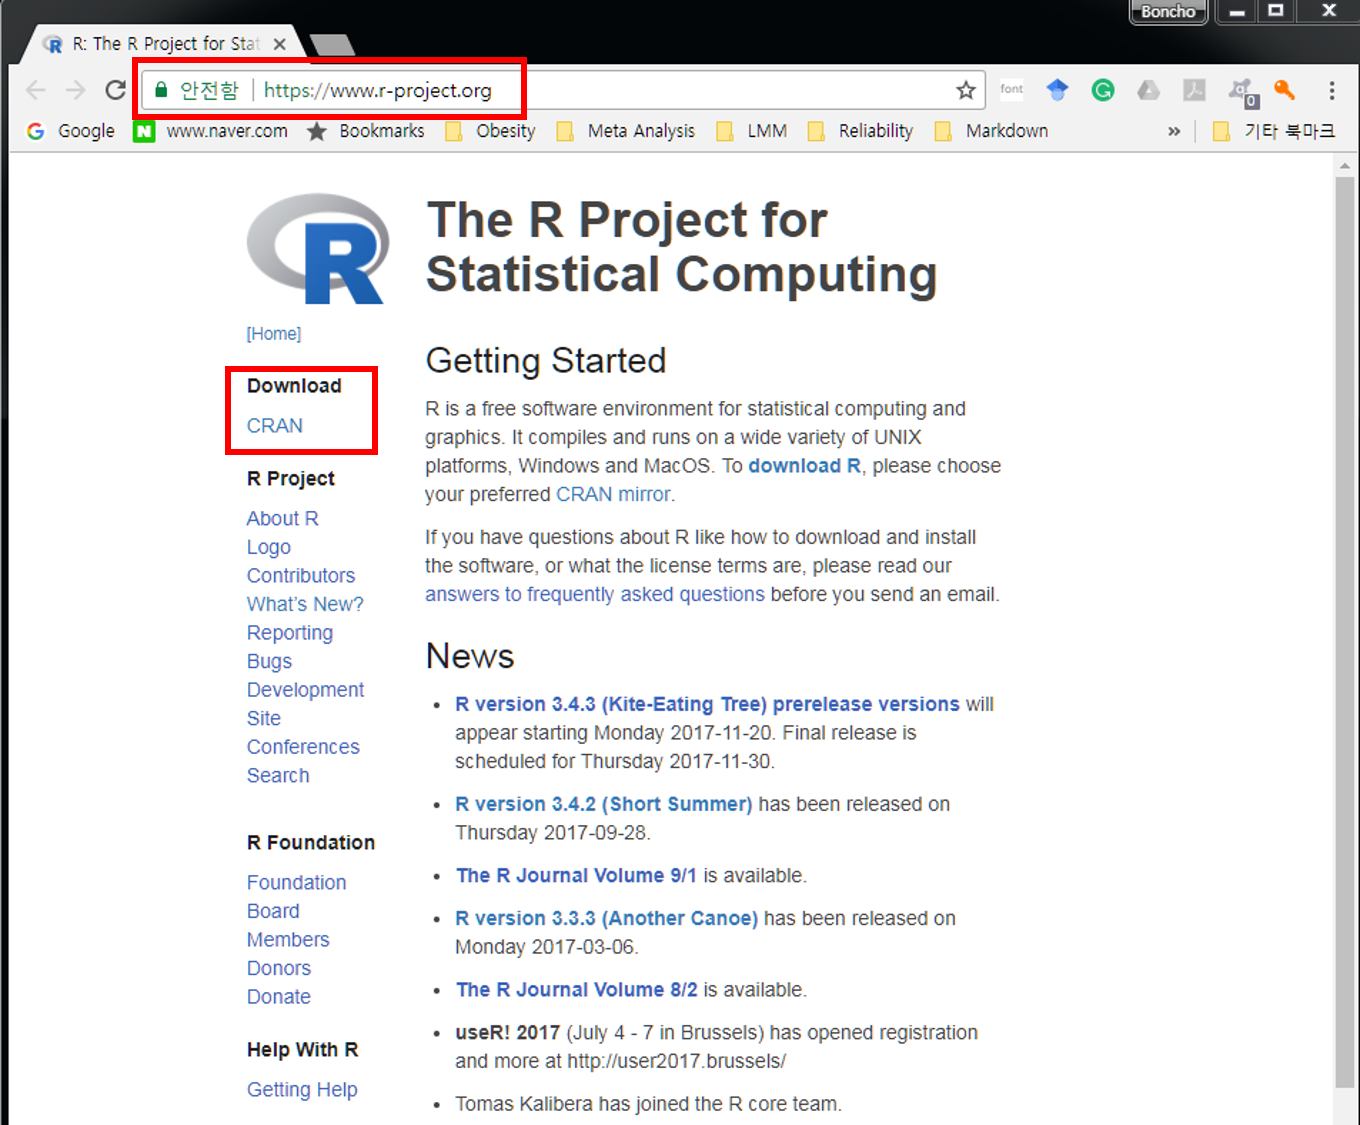
\includegraphics[width = 12cm, height = 12cm]{Figures/Rorg-main-add.png}
  \caption[www.r-project.org 메인화면]{www.r-project.org 메인화면}\label{fig:R-install-01}
}
\end{figure}

\begin{enumerate}
\def\labelenumi{\arabic{enumi}.}
\setcounter{enumi}{2}
\tightlist
\item
  클릭 후 연결 창에서 스크롤 후 ``Korea'' 아래 링크 클릭 (그림
  \ref{fig:R-install-02} 참조)
\end{enumerate}

\begin{figure}[H]
{
  \centering
  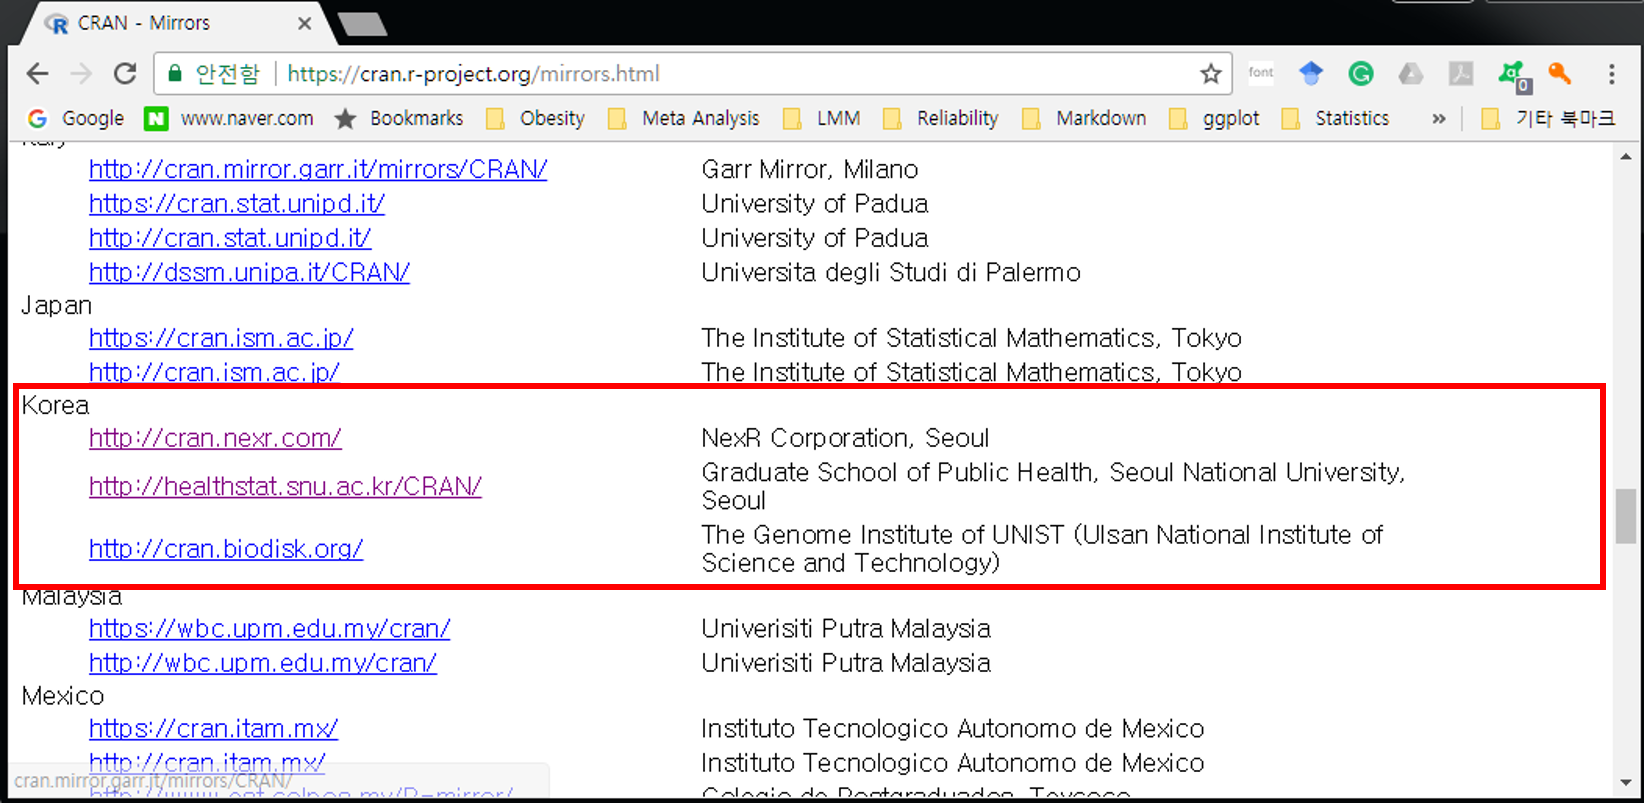
\includegraphics[width = 12cm, height = 8cm]{Figures/CRAN-korea-01.PNG}
  \caption[CRAN 국가별 mirrors]{CRAN 국가별 mirrors}\label{fig:R-install-02}
}
\end{figure}

\begin{enumerate}
\def\labelenumi{\arabic{enumi}.}
\setcounter{enumi}{3}
\tightlist
\item
  클릭 후 세 가지 운영체제(Linux, Mac OS X, Windowns)에 따른 R 버전 선택
  가능

  \begin{itemize}
  \tightlist
  \item
    본 문서에서는 Windows 버전 설치만 다룸
  \end{itemize}
\end{enumerate}

\begin{figure}[H]
{
  \centering
  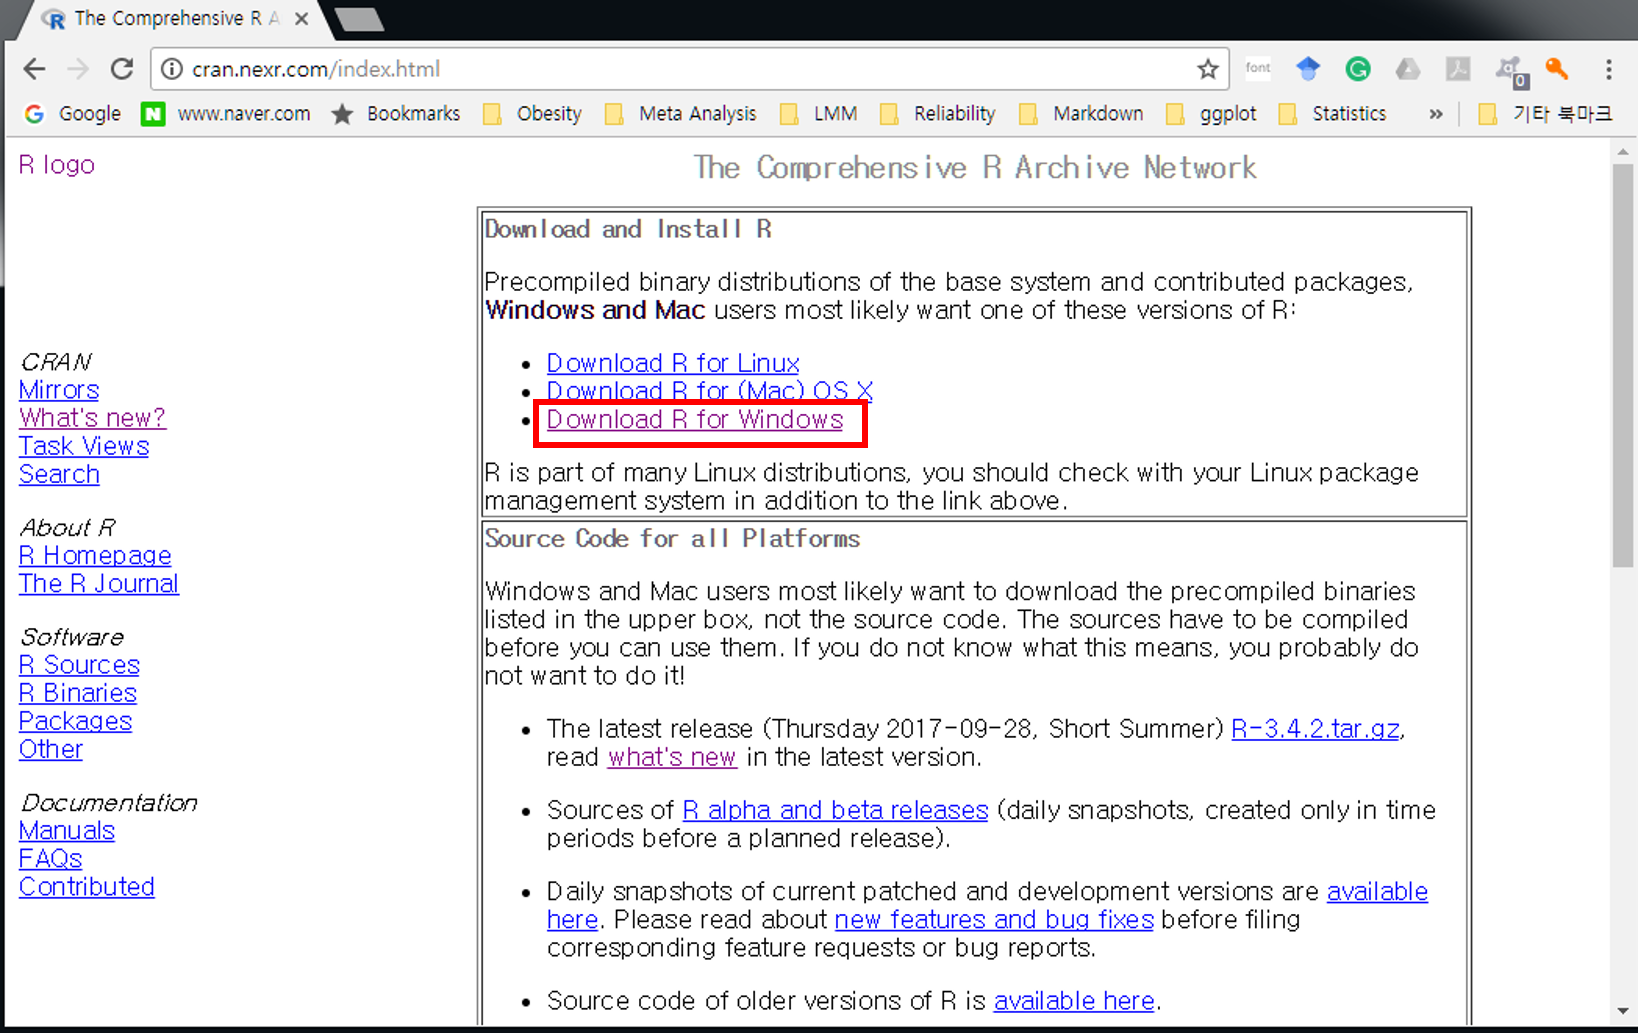
\includegraphics[width = 12cm, height = 10cm]{Figures/Rinstall-01.png}
  \caption[운영체제 별 R 버전 선택]{운영체제 별 R 버전 선택}\label{fig:R-install-03}
}
\end{figure}

\begin{enumerate}
\def\labelenumi{\arabic{enumi}.}
\setcounter{enumi}{4}
\tightlist
\item
  ``Downloads R for Windows'' 링크 클릭하면 다음과 같은 화면으로 이동
\end{enumerate}

\begin{figure}[H]
{
  \centering
  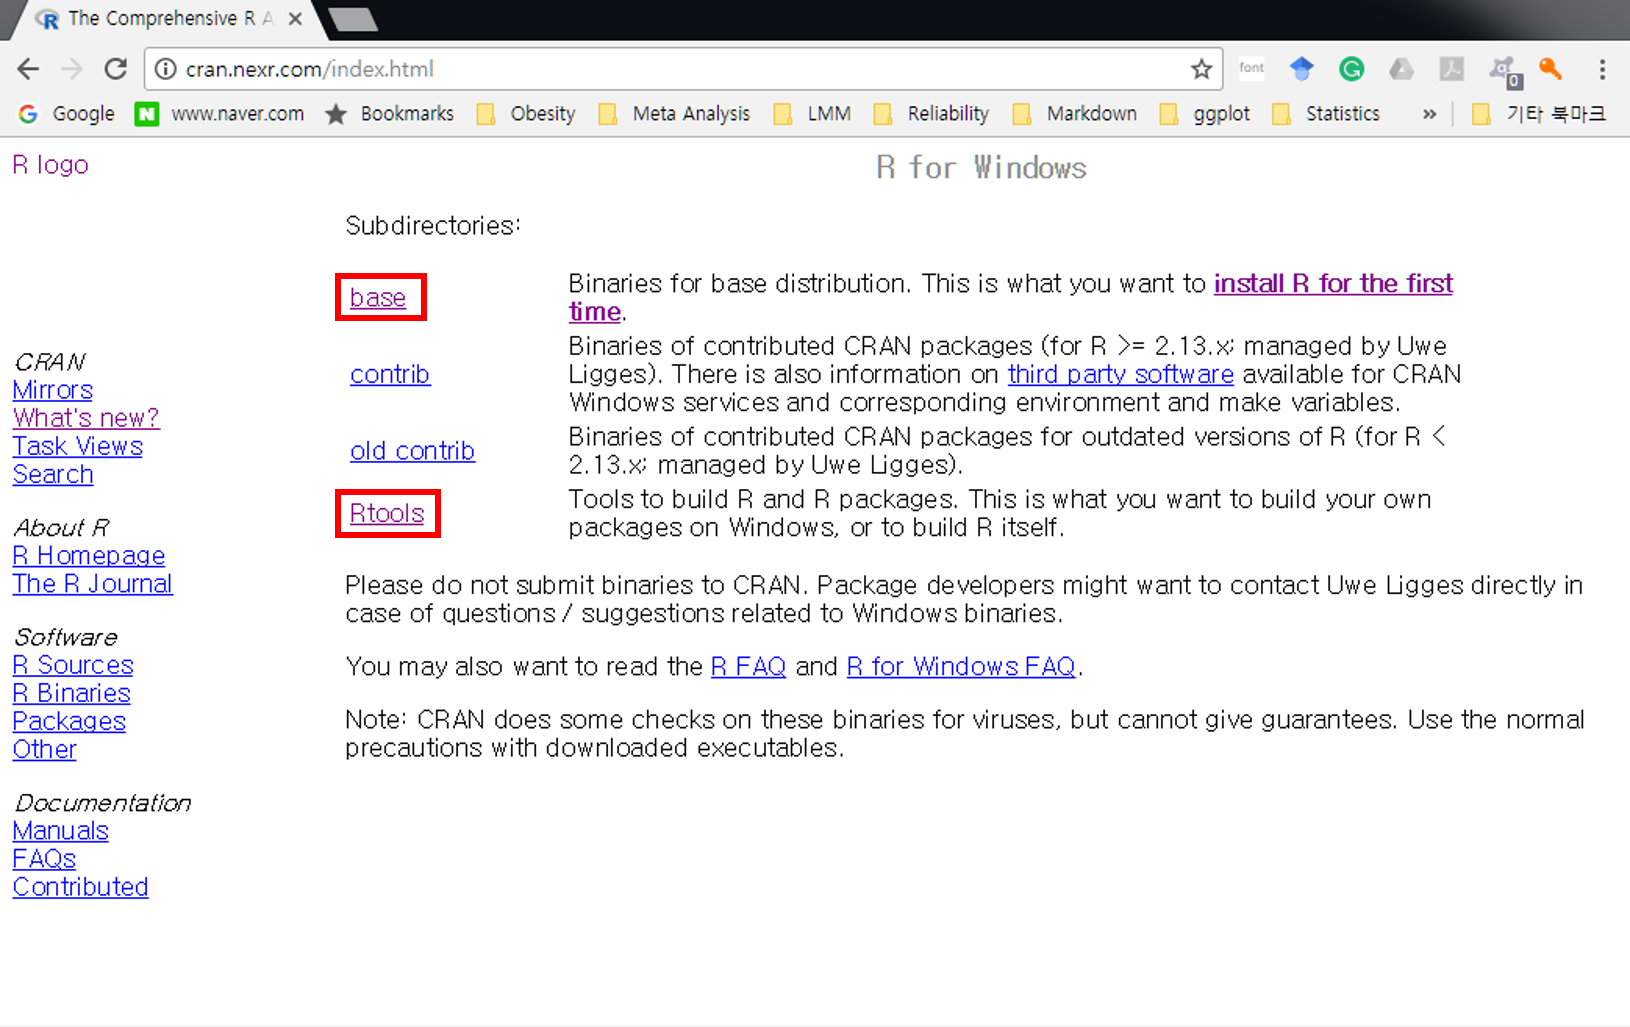
\includegraphics[width = 12cm, height = 10cm]{Figures/Rinstall-02.png}
  \caption[Windows 용 R base 및 구성요소 다운로드]{Windows 용 R base 및 구성요소 다운로드}\label{fig:R-install-04}
}
\end{figure}

\begin{enumerate}
\def\labelenumi{\arabic{enumi}.}
\setcounter{enumi}{5}
\item
  R을 구성하는 하위구조 중 ``base'' 링크 클릭 후 다음 화면에서
  ``Downloads R 3.4.2 for Windows''를 클릭 후 설치 파일을 임의의
  디렉토리에 저장 후 실행(그림 \ref{fig:R-install-05} 참조)
\item
  참고로 3개 subdirectories에 대한 간략한 설명은 아래와 같음

  \begin{itemize}
  \tightlist
  \item
    \texttt{base}: R 실행 프로그램
  \item
    \texttt{contrib}: R package의 바이너리 파일
  \item
    \texttt{Rtools}: R package 개발 및 배포를 위한 프로그램
  \end{itemize}
\end{enumerate}

\begin{figure}[H]
{
  \centering
  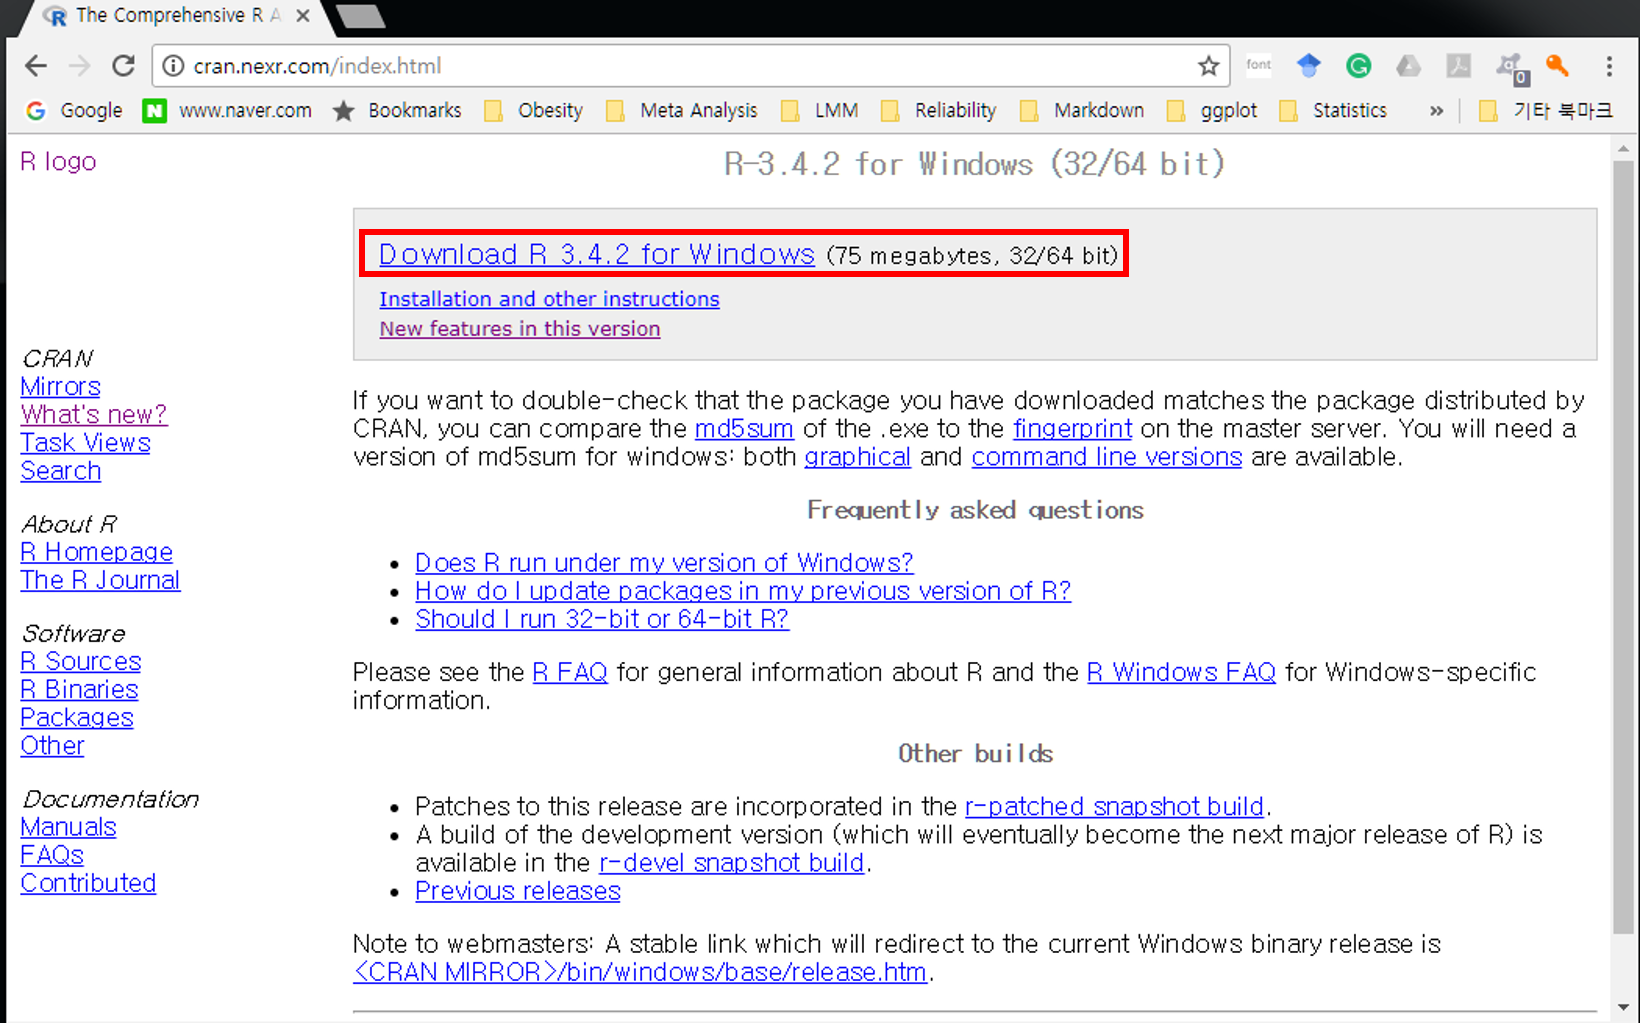
\includegraphics[width = 12cm, height = 10cm]{Figures/Rinstall-03.png}
  \caption[Windows 용 R 설치 파일 다운로드 페이지]{Windows 용 R 설치 파일 다운로드 페이지}\label{fig:R-install-05}
}
\end{figure}

\begin{enumerate}
\def\labelenumi{\arabic{enumi}.}
\setcounter{enumi}{7}
\tightlist
\item
  다운로드한 파일을 실행하면 아래와 같은 대화창이 나타남

  \begin{itemize}
  \tightlist
  \item
    한국어 선택 \(\rightarrow\) 환영 화면에서
    {[}다음(N)\textgreater{}{]} 클릭
  \end{itemize}
\end{enumerate}

\begin{figure}[H]
{
  \centering
  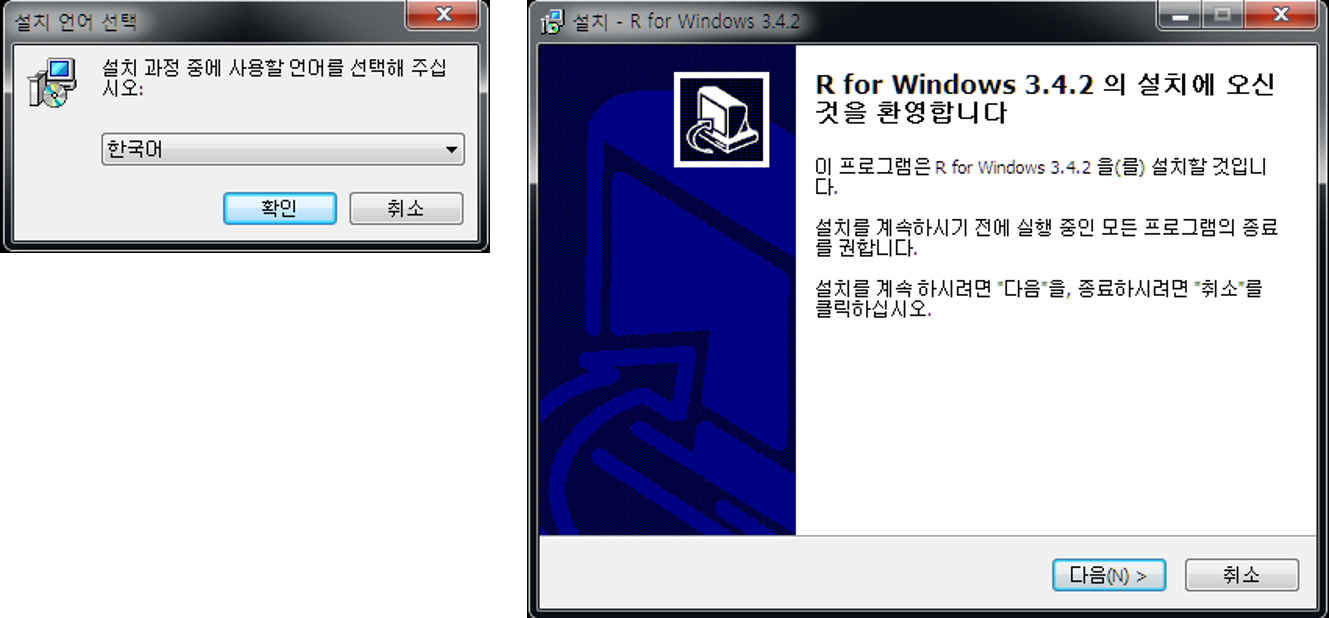
\includegraphics[width = 14cm, height = 11cm]{Figures/R-install-F01.png}
  \caption[R 설치과정 01]{R 설치과정 01}\label{fig:R-install-06}
}
\end{figure}

\begin{enumerate}
\def\labelenumi{\arabic{enumi}.}
\setcounter{enumi}{8}
\tightlist
\item
  GNU 라이센스에 대한 설명 및 동의 여부({[}다음(N)\textgreater{}{]})
  클릭 (그림 \ref{fig:R-install-07})
\end{enumerate}

\begin{figure}[H]
{
  \centering
  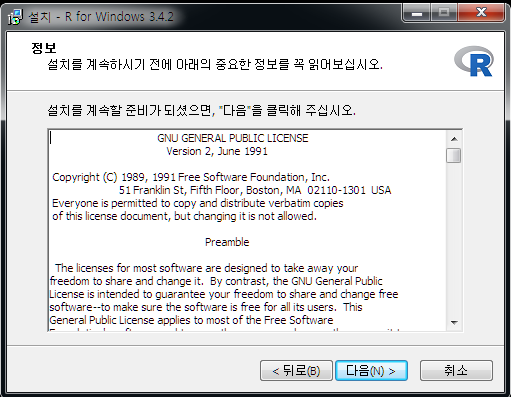
\includegraphics[width = 8cm, height = 8cm]{Figures/R-install-F02.png}
  \caption[R GNU general license]{R GNU general license}\label{fig:R-install-07}
}
\end{figure}

\begin{enumerate}
\def\labelenumi{\arabic{enumi}.}
\setcounter{enumi}{9}
\tightlist
\item
  설치 디렉토리 설정 및 구성요소 설지 여부

  \begin{itemize}
  \tightlist
  \item
    원하는 디렉토리 설정(예:
    \texttt{C:\textbackslash{}R\textbackslash{}R-3.4.2}) (그림
    \ref{fig:R-install-08})
  \item
    기본 프로그램(``Core Files''), 32 또는 64 bit 용 설치 파일, R
    console 한글 번역 모두 체크 뒤 {[}다음(N)\textgreater{}{]} 클릭
    (그림 \ref{fig:R-install-09})
  \end{itemize}
\end{enumerate}

\begin{figure}[H]
{
  \centering
  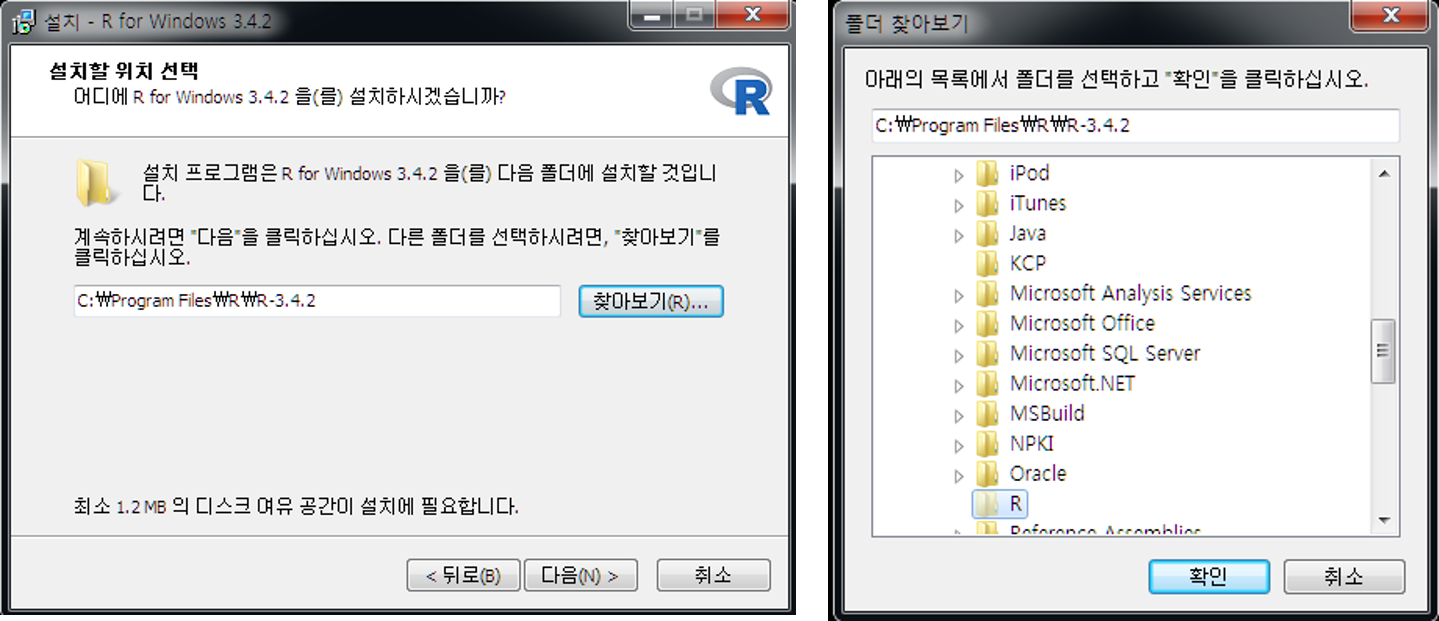
\includegraphics[width = 15cm, height = 10cm]{Figures/R-install-F03.png}
  \caption[R 설치 디렉토리 설정]{R 설치 디렉토리 설정}\label{fig:R-install-08}
}
\end{figure}

\begin{figure}[H]
{
  \centering
  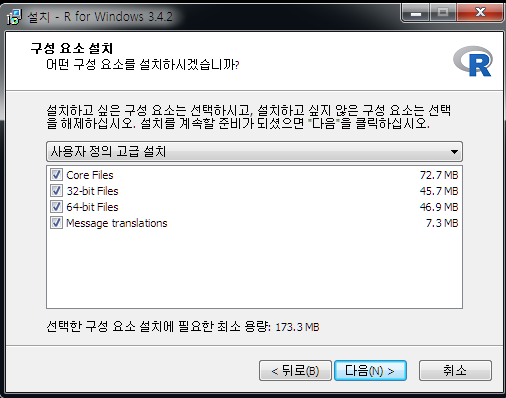
\includegraphics[width = 8cm, height = 8cm]{Figures/R-install-F04.png}
  \caption[R 구성요소 설치]{R 구성요소 설치}\label{fig:R-install-09}
}
\end{figure}

\begin{enumerate}
\def\labelenumi{\arabic{enumi}.}
\setcounter{enumi}{10}
\tightlist
\item
  R 스타트업 옵션 지정

  \begin{itemize}
  \tightlist
  \item
    기본값(``No'' check-button)으로도 설치 진행 가능
  \item
    본 문서에서는 스타트업 옵션 변경으로 진행
  \end{itemize}
\end{enumerate}

\begin{figure}[H]
{
  \centering
  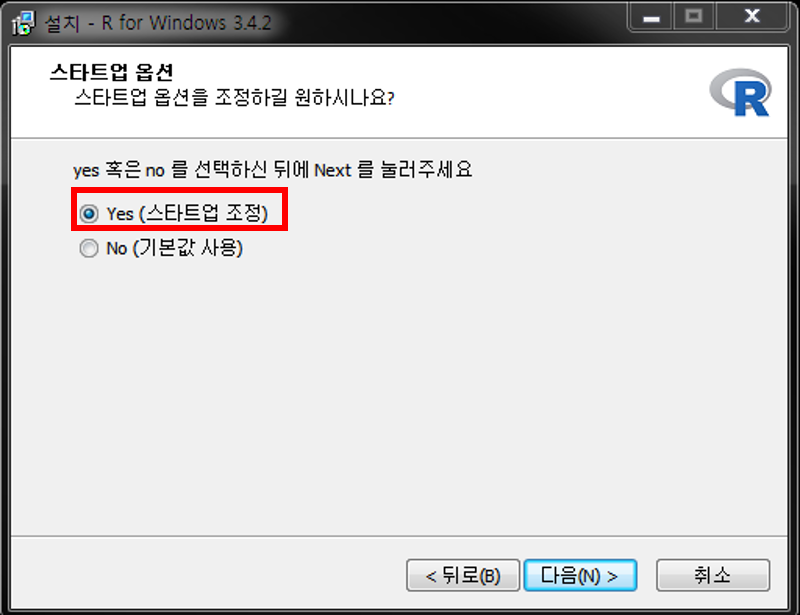
\includegraphics[width = 8cm, height = 8cm]{Figures/R-install-F05.png}
  \caption[R 스타트업 옵션 변경]{R 스타트업 옵션 변경}\label{fig:R-install-10}
}
\end{figure}

\begin{enumerate}
\def\labelenumi{\arabic{enumi}.}
\setcounter{enumi}{11}
\tightlist
\item
  화면표시방식(디스플레이 모드) 설정 변경

  \begin{itemize}
  \tightlist
  \item
    MDI: 한 윈도우 내에서 script 편집창, 출력, 도움말 창 사용
  \item
    SDI: 다중 창에서 각각 script 편집창, 출력, 도움말 등을 독립적으로
    열기
  \end{itemize}
\end{enumerate}

\begin{figure}[H]
{
  \centering
  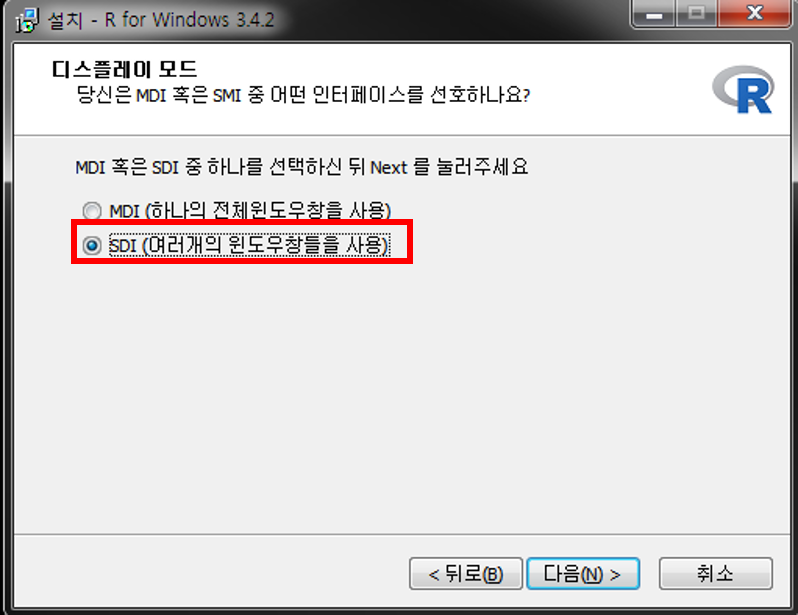
\includegraphics[width = 8cm, height = 8cm]{Figures/R-install-F06.png}
  \caption[R 화면표시방식 설정 변경]{R 화면표시방식 설정 변경}\label{fig:R-install-11}
}
\end{figure}

\begin{enumerate}
\def\labelenumi{\arabic{enumi}.}
\setcounter{enumi}{12}
\tightlist
\item
  도움말 형식에서 HTML 도움말 기반 선택
\end{enumerate}

\begin{figure}[H]
{
  \centering
  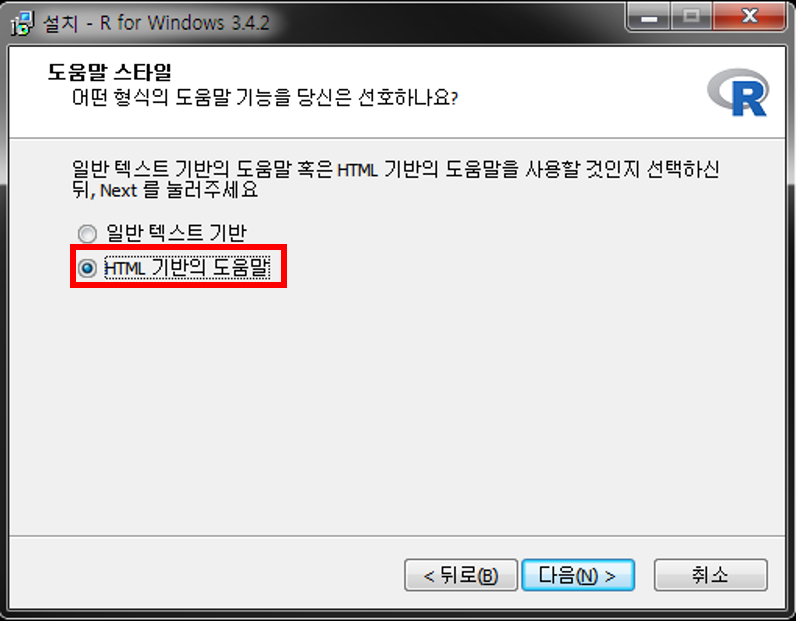
\includegraphics[width = 8cm, height = 8cm]{Figures/R-install-F07.png}
  \caption[R 도움말 형식 변경]{R 도움말 형식 변경}\label{fig:R-install-12}
}
\end{figure}

\begin{enumerate}
\def\labelenumi{\arabic{enumi}.}
\setcounter{enumi}{13}
\tightlist
\item
  시작메뉴 폴더 선택(그림 \ref{fig:R-install-13})

  \begin{itemize}
  \tightlist
  \item
    ``바로가기''를 생성할 시작 메뉴 폴더 지정 후
    {[}다음(N)\textgreater{}{]} 클릭 후 설치 진행
  \item
    하단 ``시작메뉴 폴더 만들지 않음'' 체크박스 표시 시 시작메뉴에
    ``바로가기'' 생성되지 않음(실행에 전혀 지장 없음)
  \end{itemize}
\end{enumerate}

\begin{figure}[H]
{
  \centering
  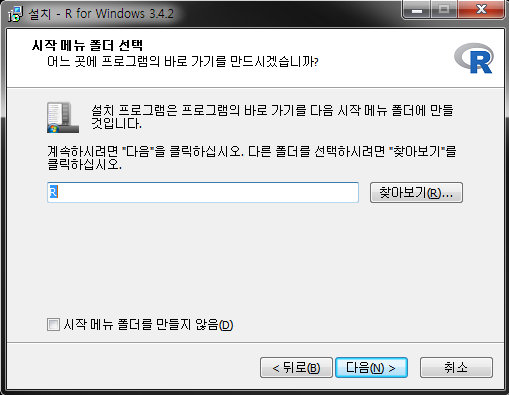
\includegraphics[width = 8cm, height = 8cm]{Figures/R-install-F08.png}
  \caption[시작메뉴 폴더 선택]{시작메뉴 폴더 선택}\label{fig:R-install-13}
}
\end{figure}

\begin{enumerate}
\def\labelenumi{\arabic{enumi}.}
\setcounter{enumi}{14}
\tightlist
\item
  추가 옵션 지정: 바탕화면 아이콘 생성 등 추가적 작업 옵션 체크 후
  {[}다음(N)\textgreater{}{]} 클릭 \(\rightarrow\) 설치 진행

  \begin{itemize}
  \tightlist
  \item
    설치된 R 버전 정보 레지스트리 저장 여부
  \item
    \texttt{.Rdata} 확장자를 R 실행파일과 자동 연계
  \end{itemize}
\end{enumerate}

\begin{figure}[H]
{
  \centering
  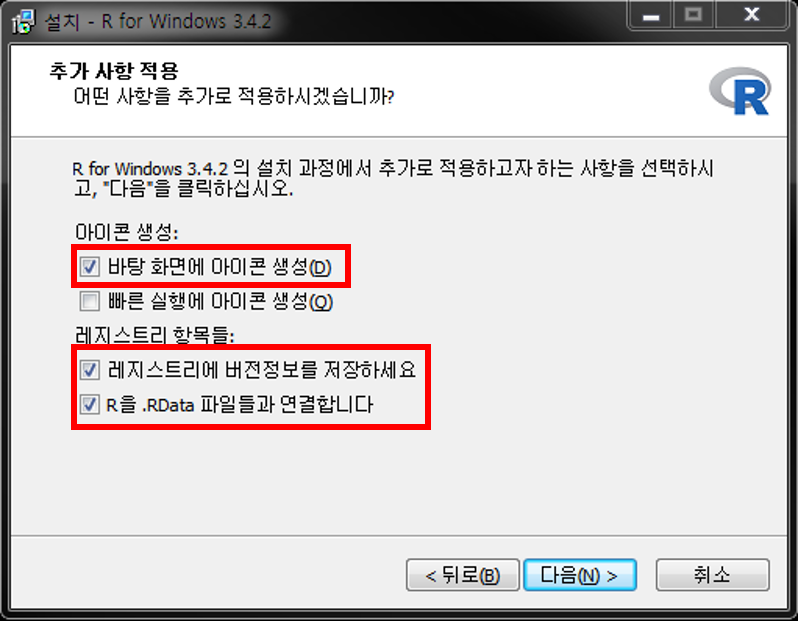
\includegraphics[width = 8cm, height = 8cm]{Figures/R-install-F09.png}
  \caption[R 추가옵션 사항 선택]{R 추가옵션 사항 선택}\label{fig:R-install-14}
}
\end{figure}

\begin{enumerate}
\def\labelenumi{\arabic{enumi}.}
\setcounter{enumi}{15}
\tightlist
\item
  설치 완료 후 바탕화면의 R 아이콘을 더블클릭하면 Rgui가 실행
\end{enumerate}

\begin{figure}[H]
{
  \centering
  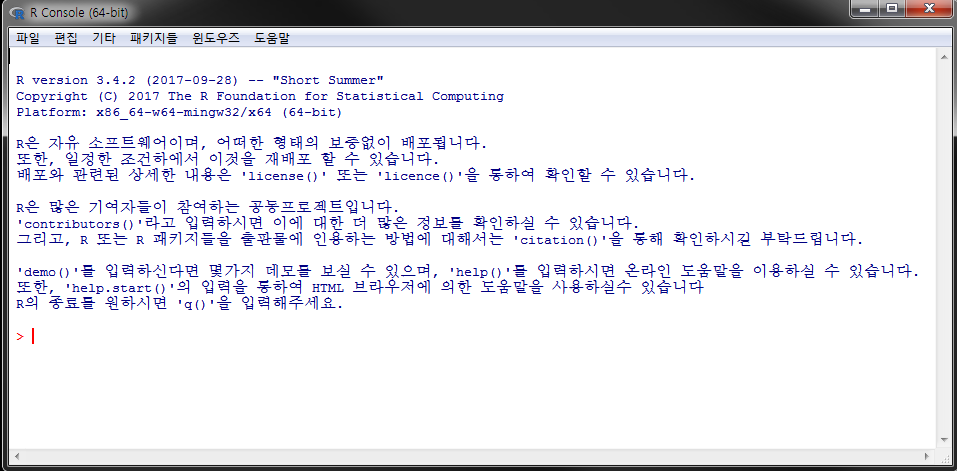
\includegraphics[width = 15cm, height = 10cm]{Figures/Rgui.png}
  \caption[Windows에서 R 실행화면(SDI)]{Windows에서 R 실행화면(콘솔 창, SDI 모드)}\label{fig:R-install-15}
}
\end{figure}

\section{R 시작 및 작동 체크}\label{r----}

위 R 시작화면에서 간단한 명령어들을 체크

\begin{itemize}
\tightlist
\item
  그림 \ref{fig:R-install-15}에서 \texttt{\textgreater{}} 기호는 R의
  명령 프롬프트임.
\item
  Checklist

  \begin{enumerate}
  \def\labelenumi{\arabic{enumi})}
  \tightlist
  \item
    ``Hello R'' 출력
  \item
    1부터 100까지 정수 출력
  \item
    간단한 histogram 출력
  \end{enumerate}
\end{itemize}

\begin{Shaded}
\begin{Highlighting}[]
\OperatorTok{>}\StringTok{ }\CommentTok{# 문자열 출력}
\ErrorTok{>}\StringTok{ }\KeywordTok{print}\NormalTok{(}\StringTok{"Hello R"}\NormalTok{)}
\end{Highlighting}
\end{Shaded}

\begin{verbatim}
[1] "Hello R"
\end{verbatim}

여기서 \texttt{\#} 기호는 주석의 시작을 의미하며 같은 행에서 \texttt{\#}
뒤 내용의 코드는 실행되지 않음

\begin{Shaded}
\begin{Highlighting}[]
\OperatorTok{>}\StringTok{ }\CommentTok{# 1부터 100까지 수열 출력}
\ErrorTok{>}\StringTok{ }\KeywordTok{seq}\NormalTok{(}\DecValTok{1}\OperatorTok{:}\DecValTok{100}\NormalTok{)  }\CommentTok{# print('Hello R')}
\end{Highlighting}
\end{Shaded}

\begin{verbatim}
  [1]   1   2   3   4   5   6   7   8   9  10  11  12  13  14  15  16  17
 [18]  18  19  20  21  22  23  24  25  26  27  28  29  30  31  32  33  34
 [35]  35  36  37  38  39  40  41  42  43  44  45  46  47  48  49  50  51
 [52]  52  53  54  55  56  57  58  59  60  61  62  63  64  65  66  67  68
 [69]  69  70  71  72  73  74  75  76  77  78  79  80  81  82  83  84  85
 [86]  86  87  88  89  90  91  92  93  94  95  96  97  98  99 100
\end{verbatim}

\begin{Shaded}
\begin{Highlighting}[]
\OperatorTok{>}\StringTok{ }\CommentTok{# 간단한 히스토그램}
\ErrorTok{>}\StringTok{ }\KeywordTok{set.seed}\NormalTok{(}\DecValTok{12345}\NormalTok{)  }\CommentTok{# random seed 지정}
\OperatorTok{>}\StringTok{ }\NormalTok{x <-}\StringTok{ }\KeywordTok{rnorm}\NormalTok{(}\DecValTok{1000}\NormalTok{)  }\CommentTok{# 평균 0, 분산 1인 정규분포에서 난수 1000개 생성}
\OperatorTok{>}\StringTok{ }\KeywordTok{hist}\NormalTok{(x)  }\CommentTok{# 히스토그램}
\end{Highlighting}
\end{Shaded}

\begin{center}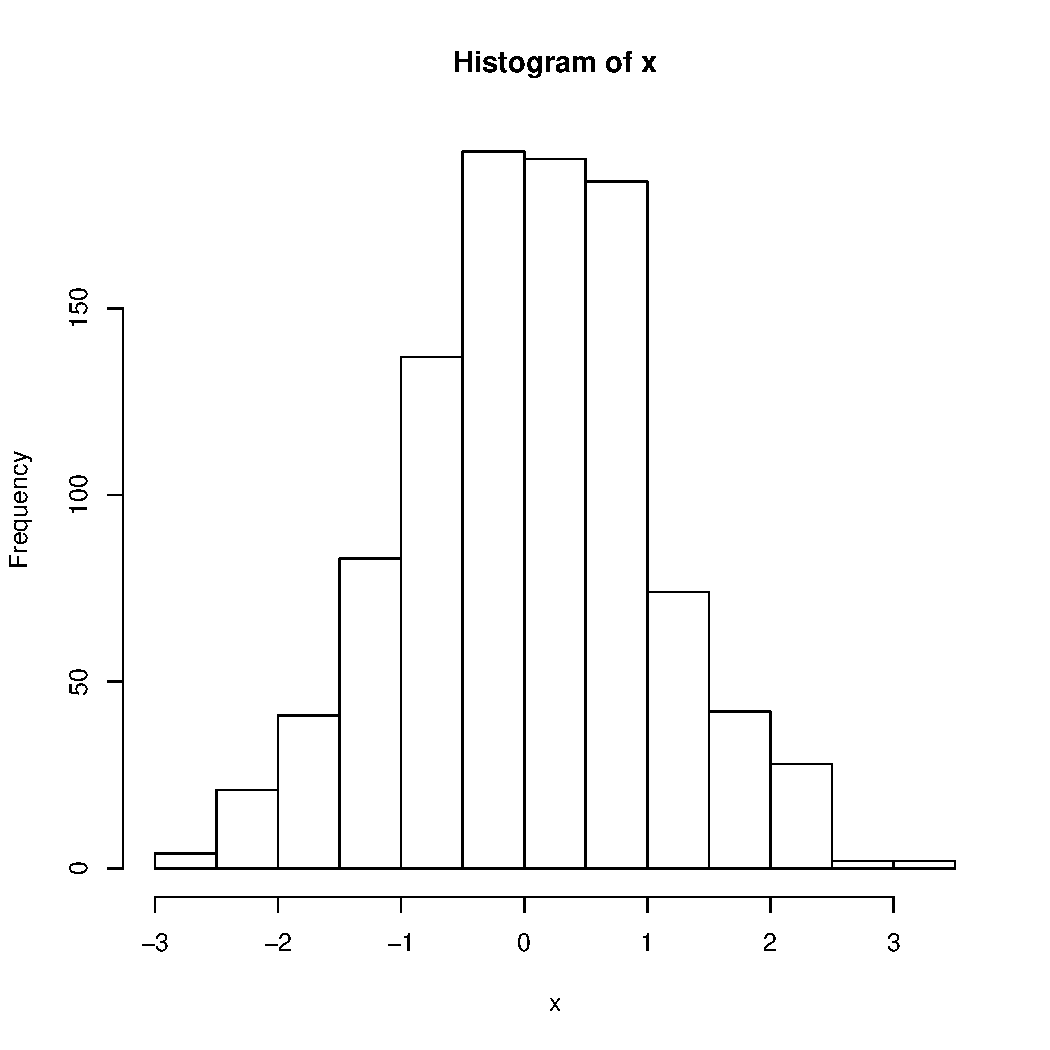
\includegraphics[width=10 cm,height=10 cm]{Figures/check-03-1} \end{center}

\begin{quote}
\colorbox{gray!10}{\begin{minipage}{15cm}
\textbf{Tips}

R 명령어 실행 시 간혹 아니 매우 빈번히 오류가 나타나는데, 이를 해결할 수 있는 가장 손쉬운 방법은 Googling과 R의 도움말을 이용하는 것이 가장 효율적임. 
\end{minipage}}
\end{quote}

도움말을 볼 수 있은 R 함수 리스트

\begin{table}[H]
  \centering
  \begingroup\footnotesize
  \caption{R help 관련 명령어 리스트}
  \begin{tabular}{p{3cm}p{5cm}p{7cm}}
  \toprule
  \textbf{도움말 보기 명령어} & \textbf{설명} & \textbf{사용법} \\
  \midrule
  \texttt{help} 또는 \texttt{?}          & 도움말 시스템 호출               & \texttt{help(topic \textit{\# 도움말을 찾고자 하는 대상 또는 함수}) }\\
  \texttt{help.search} 또는 \texttt{??}  & 주어진 문자열을 포함한 문서 검색 & \texttt{help.search(pattern \textit{\# 찾고자 하는 문자열})} \\ 
  \texttt{example}                       & topic의 도움말 페이지에 있는 examples section 실행 & \texttt{example(topic \textit{\# 예제를 실행하고자 하는 topic 또는 함수})} \\
  \texttt{vignette}                      & topic의 pdf 또는 html 레퍼런스 메뉴얼 불러오기 & \texttt{vignette(topic \textit{\# topic에 저장된 reference manual})} \\
  \bottomrule
  \end{tabular}
  \endgroup
\end{table}

\subsection{이것으로 R 설치 완료??}\label{-r--}

\begin{itemize}
\tightlist
\item
  기본적 R 사용방식은 입력한 명령어와 실행결과를 확인하는
  대화형(interpreter) 방식
\item
  R 기본 콘솔창 안에서도 \keystroke{TAB}을 누르면 자동완성 기능이라던가
  \keystroke{$\uparrow$}, \keystroke{$\downarrow$}를 누르면 이전/이후
  명령 기록을 볼 수 있음.
\item
  여러 줄 이상의 R 명령어라든가 반복적, 장기간 작업을 수행해야 하는
  경우라면 R 명령어로 구성된 스크립트 작성 후 일괄 실행하는 것이
  일반적임.
\item
  이러한 다중 명령 코딩 시 콘솔창에 직접 입력하는 것은 비효율적
  \(\rightarrow\) 스크립트 에디터를 주로 사용
\item
  R 자체적으로 기본적인 스크립트 에디터 제공(R editor) \(\rightarrow\)
  가독성 및 코딩 효율이 떨어짐
\item
  대표적 R 에디터: WinEdt (\url{http://www.winedt.com}), Tinn-R
  (\url{https://sourceforge.net/projects/tinn-r/}), Vim
  (\url{http://www.vim.org/scripts/script.php?script_id=2628})
\item
  대부분의 분석 및 개발 환경이 RGUI 만으로 구성되어 있지 않음
  \(\rightarrow\) \textbf{RStudio}를 이용한 통합 분석 환경 설정
\end{itemize}

\newpage

\section{RStudio 설치하기}\label{rstudio-}

\begin{itemize}
\tightlist
\item
  Rstudio: R 통합 분석/개발 환경(integrated development environment,
  IDE)으로 현재 가장 대중적으로 사용되고 있는 R 사용 환경
\item
  명령 콘솔 외 파일 편집, 데이터 보기, 명령 기록(\texttt{.history}),
  그래프 등에 쉽게 접근 가능
\item
  R과 마찬가지로 무료 소프트웨어임
\end{itemize}

\begin{enumerate}
\def\labelenumi{\arabic{enumi}.}
\tightlist
\item
  Rstudio 사이트 접속

  \begin{itemize}
  \tightlist
  \item
    웹 브라우저를 통해 \url{https://www.rstudio.com} 연결 후 메인
    화면에서 ``Download Rstudio'' 클릭
  \item
    혹은 상단 Pop-up manu 중 Products \(\rightarrow\) RStudio 클릭 후
    연결된 화면에서 다운로드 진행
  \end{itemize}
\end{enumerate}

\begin{figure}[H]
{
  \centering
  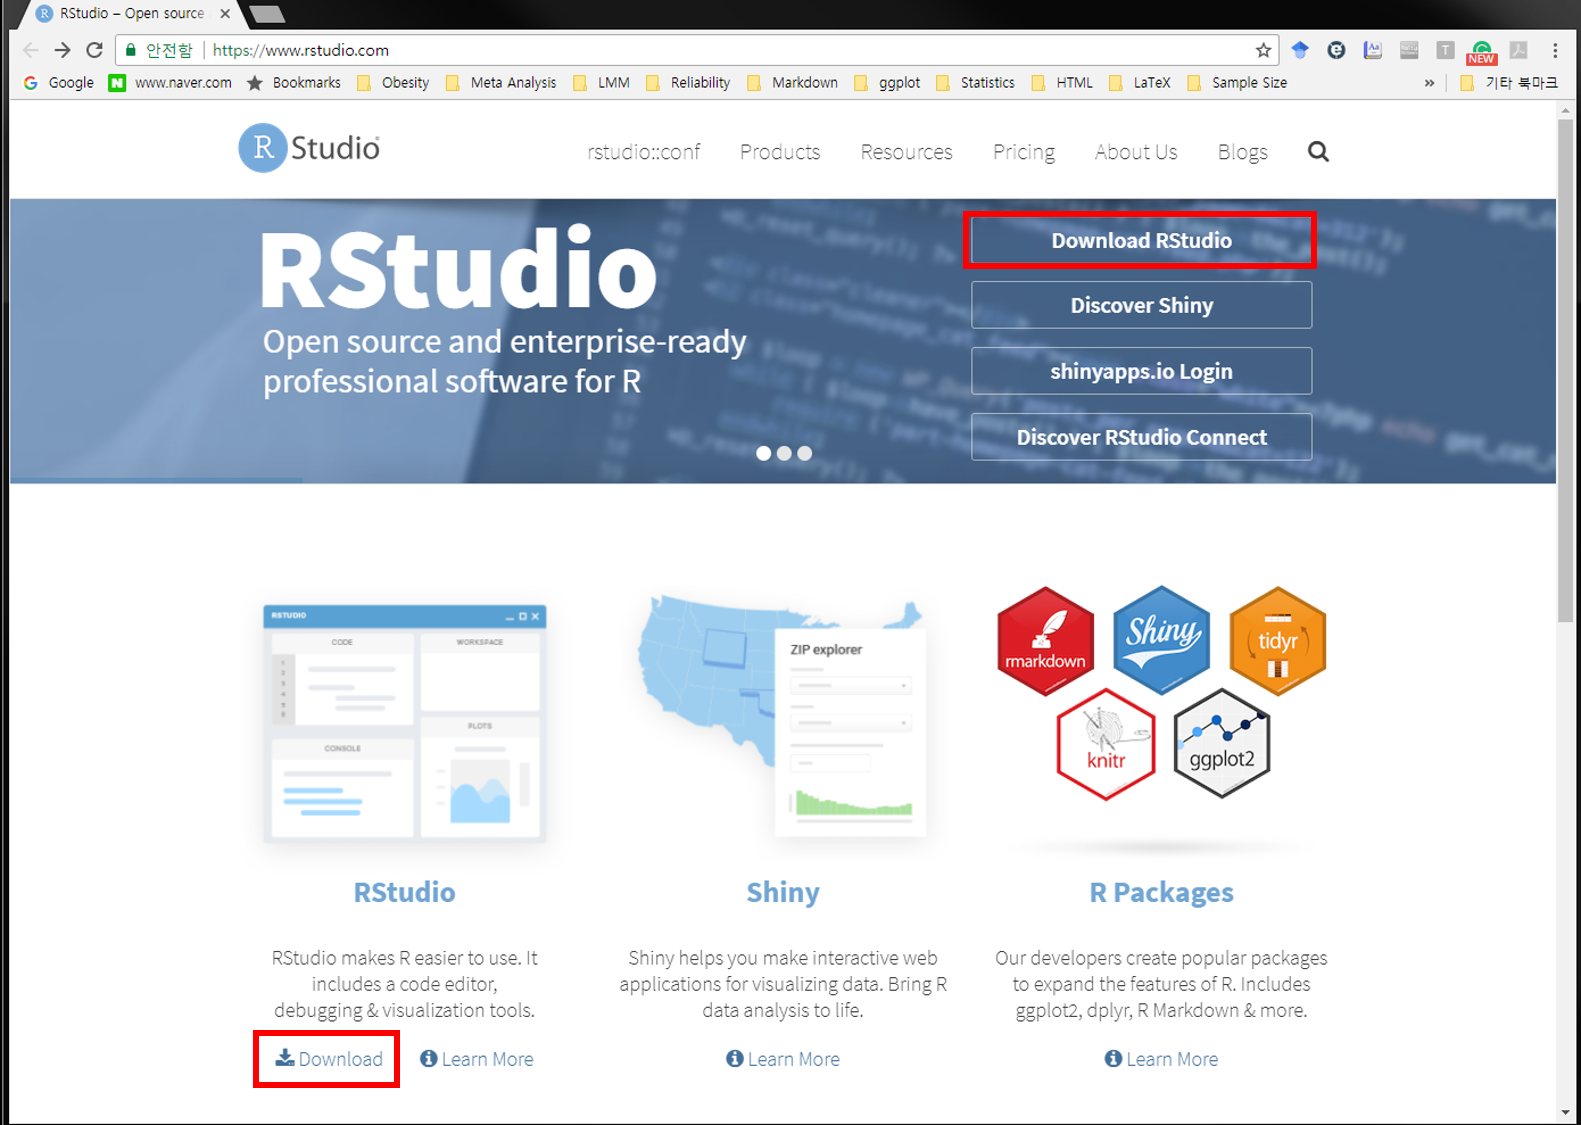
\includegraphics[width = 13cm, height = 13cm]{Figures/Rstudio-main.png}
  \caption[RStudio 메인 페이지]{RStudio 메인 페이지 화면}\label{fig:Rstudio-install-01}
}
\end{figure}

\begin{enumerate}
\def\labelenumi{\arabic{enumi}.}
\setcounter{enumi}{1}
\tightlist
\item
  Desktop 또는 Sever 버전 중 택일

  \begin{itemize}
  \tightlist
  \item
    서버용 설치를 위해서는 Server 클릭 \(\rightarrow\) 소규모 자료
    분석용으로는 불필요
  \item
    여기서는 ``Desktop'' 버전 선택 후 다음 링크로 이동
  \end{itemize}
\end{enumerate}

\begin{figure}[H]
{
  \centering
  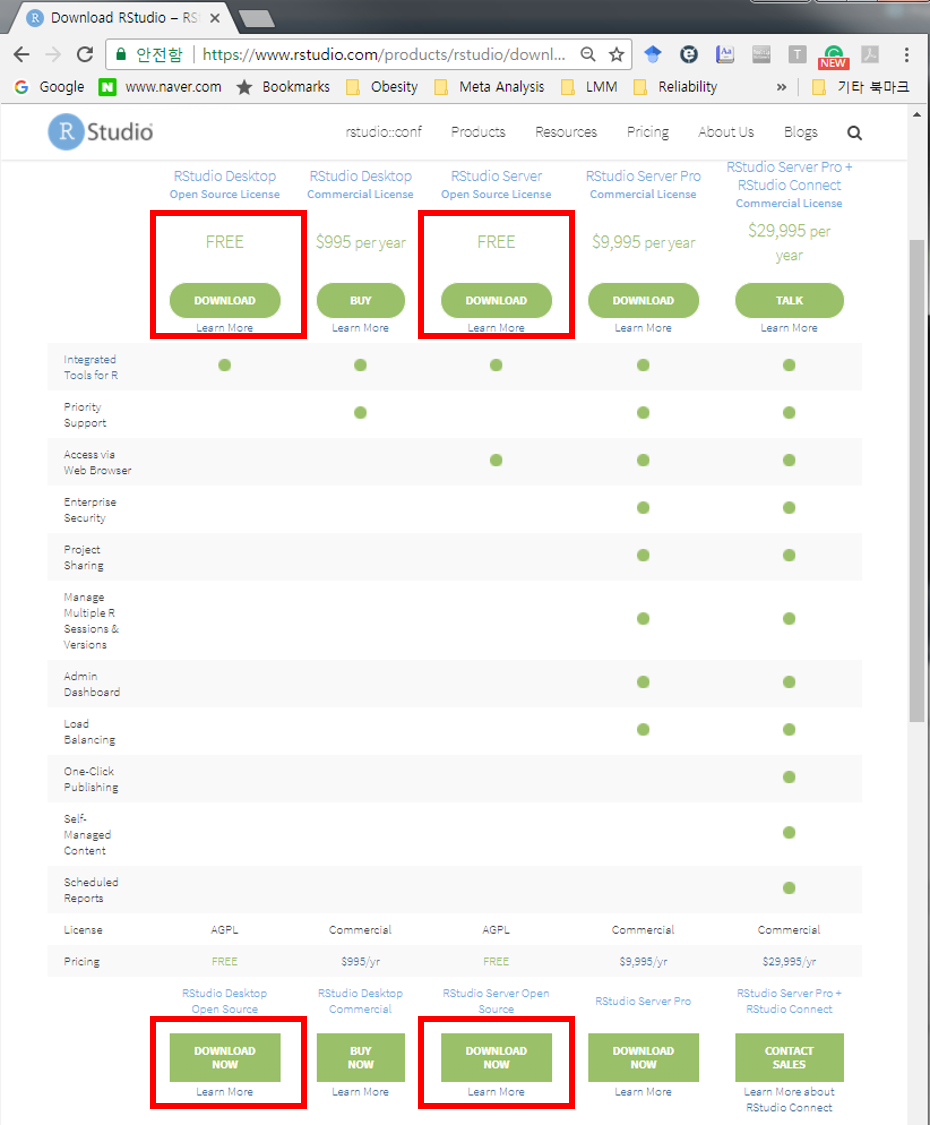
\includegraphics[width = 12cm, height = 10cm]{Figures/Rstudio-download.png}
  \caption[RStudio 다운로드 페이지]{RStudio 다운로드 페이지}\label{fig:Rstudio-install-02}
}
\end{figure}

\begin{enumerate}
\def\labelenumi{\arabic{enumi}.}
\setcounter{enumi}{2}
\tightlist
\item
  운영체제에 맞는 Rstudio installer 다운로드(여기서는 Windows 버전
  다운로드)
\end{enumerate}

\begin{figure}[H]
{
  \centering
  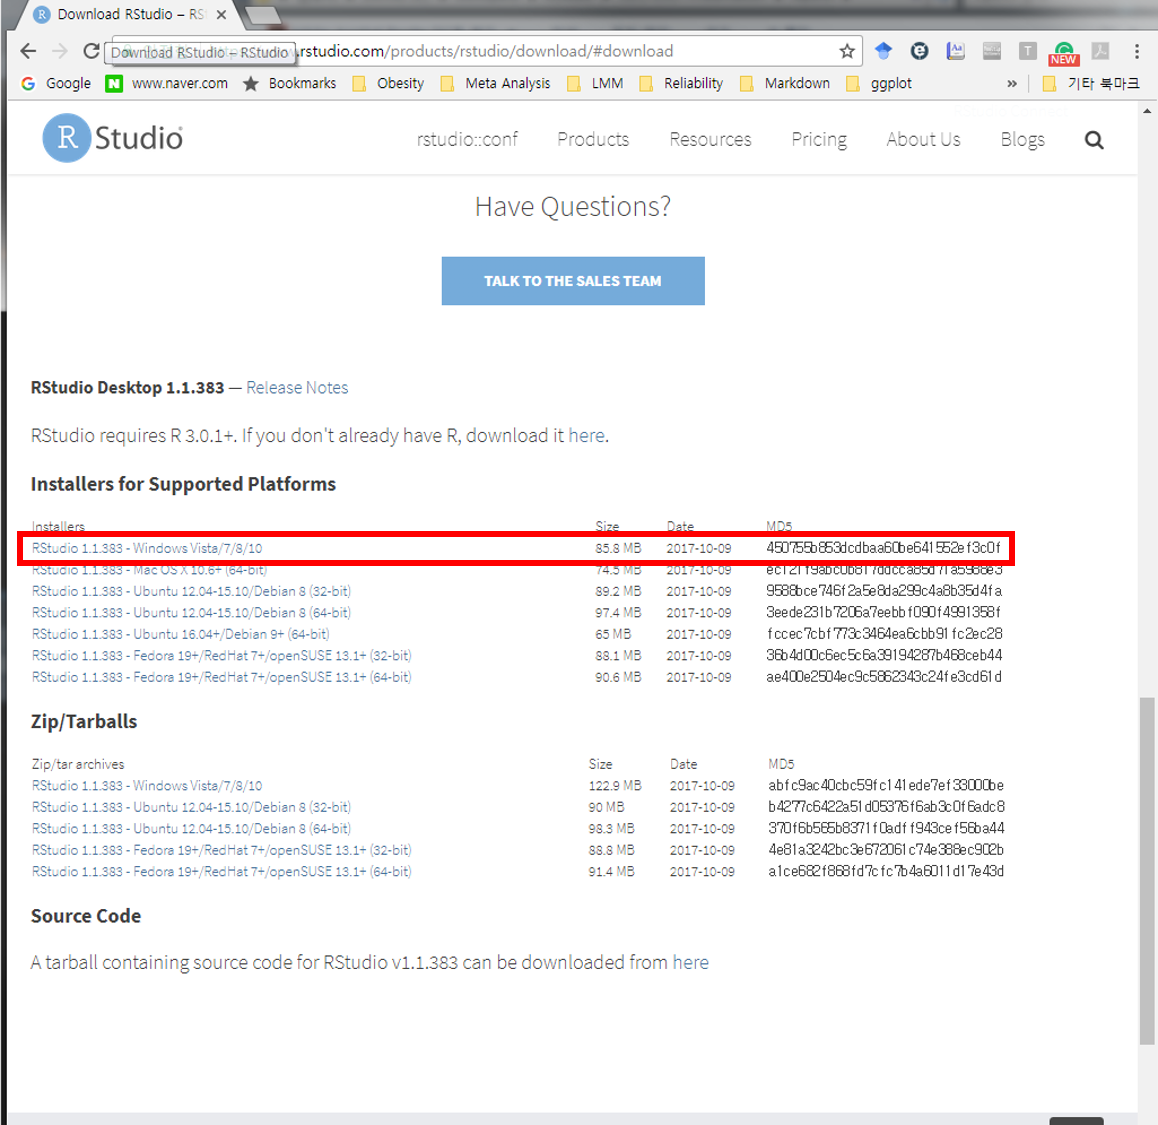
\includegraphics[width = 12cm, height = 10cm]{Figures/Rstudio-download-02.png}
  \caption[RStudio 운영체제 선택]{RStudio 운영체제 선택}\label{fig:Rstudio-install-03}
}
\end{figure}

\begin{enumerate}
\def\labelenumi{\arabic{enumi}.}
\setcounter{enumi}{3}
\tightlist
\item
  RStudio installer 다운로드 시 파일이 저장된 폴더에서 보통
  \texttt{RStudio-xx.xx.xxx.exe} 형식의 파일명 확인

  \begin{itemize}
  \tightlist
  \item
    더블 클릭 후 실행
  \item
    \keystroke{다음>} 몇 번 누르면 설치 종료
  \end{itemize}
\end{enumerate}

\begin{figure}[H]
{
  \centering
  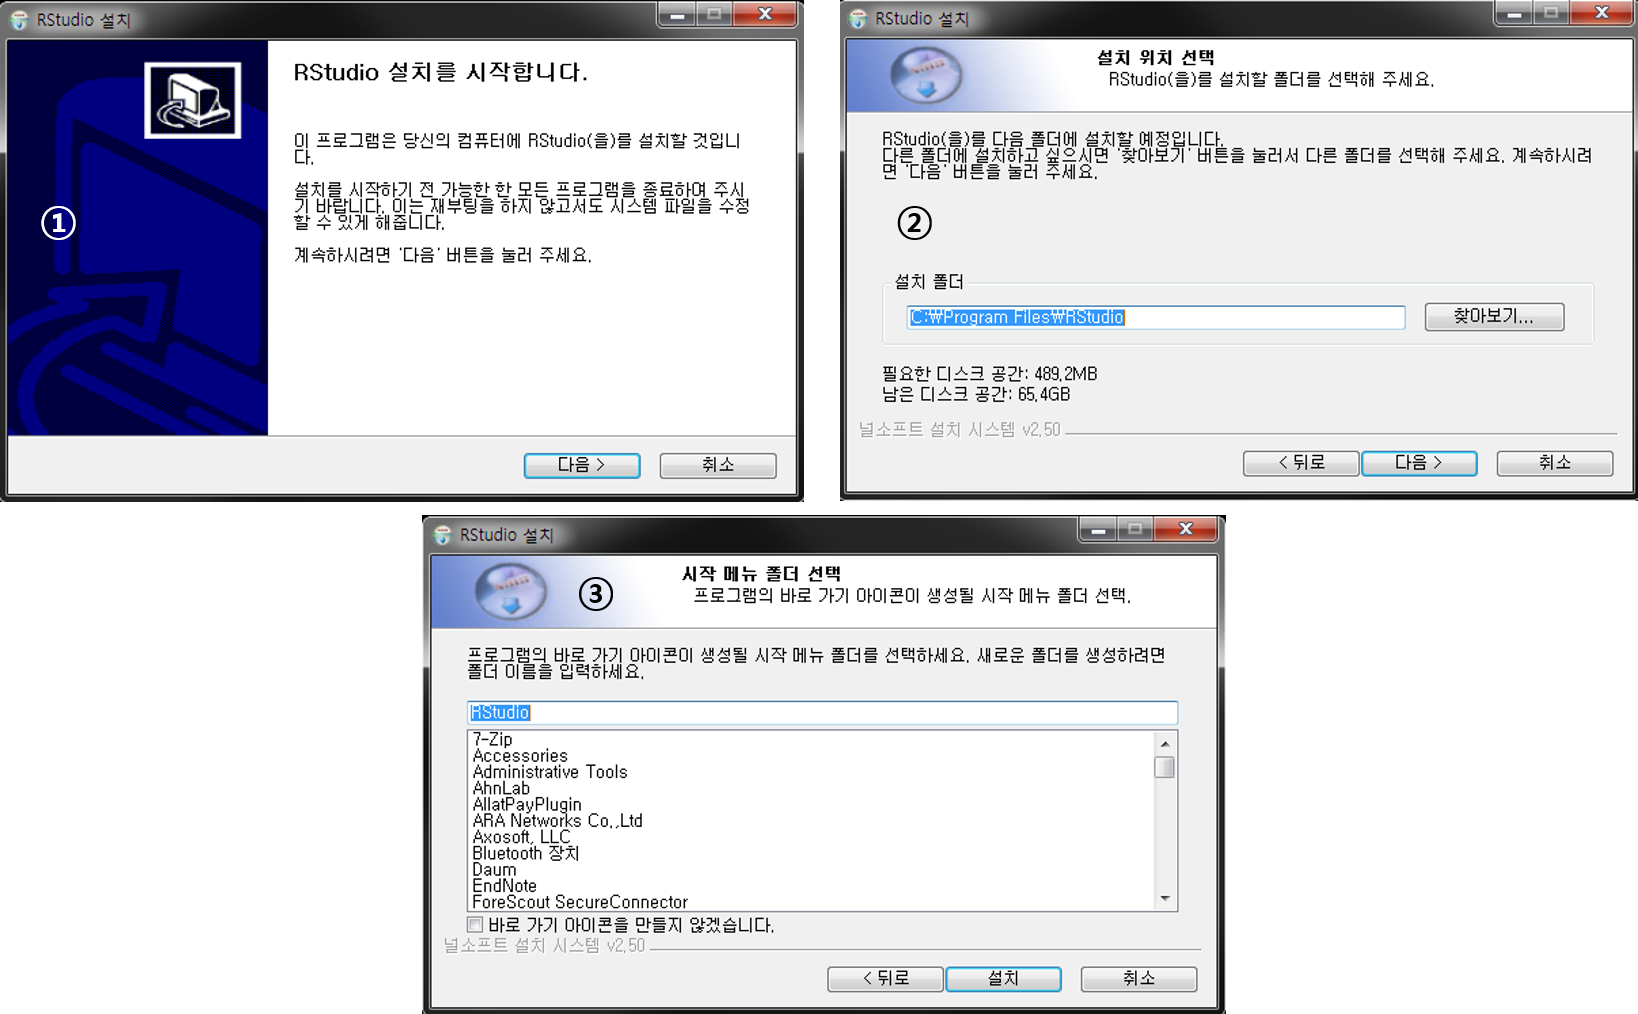
\includegraphics[width = 15cm, height = 12cm]{Figures/Rstudio-installer.png}
  \caption[RStudio 설치화면]{RStudio 설치화면}\label{fig:Rstudio-install-04}
}
\end{figure}

\begin{enumerate}
\def\labelenumi{\arabic{enumi}.}
\setcounter{enumi}{4}
\tightlist
\item
  아래와 같은 실행화면이 나타나면 RStudio 설치 성공
\end{enumerate}

\begin{figure}[H]
{
  \centering
  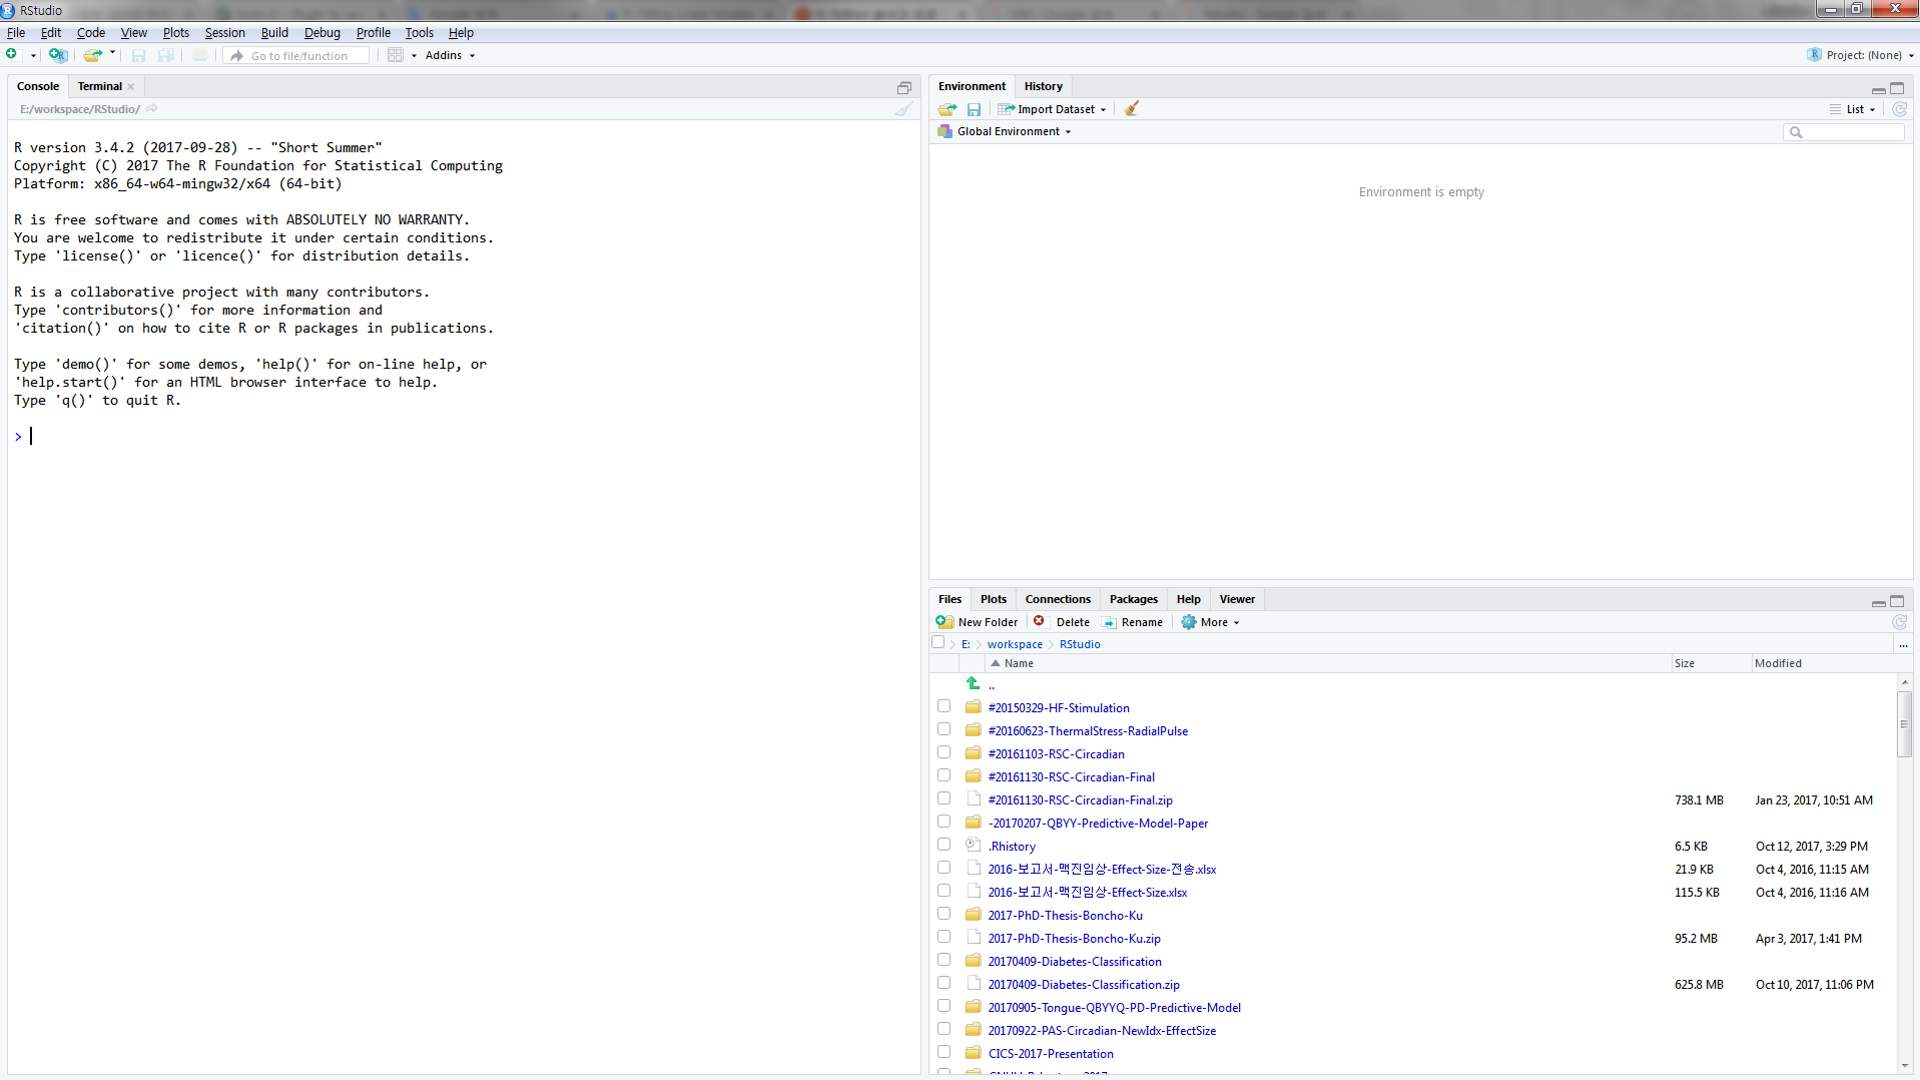
\includegraphics[width = 15cm, height = 13cm]{Figures/Rstudio-init.png}
  \caption[RStudio 초기 실행화면]{RStudio 초기 실행화면}\label{fig:Rstudio-install-05}
}
\end{figure}

\section{RStudio 튜닝}\label{rstudio-}

\begin{enumerate}
\def\labelenumi{\arabic{enumi}.}
\tightlist
\item
  RStudio IDE 화면 구성: 아래 그림 \ref{fig:Rstudio-part-01}과 같이 크게
  4개 창으로 구성

  \begin{enumerate}
  \def\labelenumii{\arabic{enumii})}
  \tightlist
  \item
    콘솔(console)

    \begin{itemize}
    \tightlist
    \item
      R 명령어 실행 공간(RGui, 정확하게는 \texttt{Rterm.exe}가 실행되고
      있는 창)
    \item
      R 스크립트 또는 콘솔 창에서 작성한 명령어(프로그램) 실행 결과 출력
    \item
      경고, 에러/로그 등의 메세지 확인
    \end{itemize}
  \item
    스크립트(script)

    \begin{itemize}
    \tightlist
    \item
      명령어의 일괄처리(batch processing)
    \item
      \keystroke{Ctrl} + \keystroke{Enter}: 선택한 블럭 내 명령어 실행
    \item
      \keystroke{Alt} + \keystroke{Enter}: 선택 없이 커서가 위치한
      라인의 명령어 실행
    \item
      \keystroke{Ctrl} + \keystroke{Alt} + \keystroke{R} 또는
      \keystroke{Ctrl} + \keystroke{Shift} + \keystroke{Enter}:
      실행하고자 하는 R 명령어들이 저장된 배치파일(\texttt{filename.R})
      일괄실행(콘솔에 실행 명령어 출력)
    \item
      \keystroke{Ctrl} + \keystroke{Shift} + \keystroke{S}: 위 작업을
      실행 명령어 출력 없이 실행

      \begin{figure}[H]
      {
        \centering
        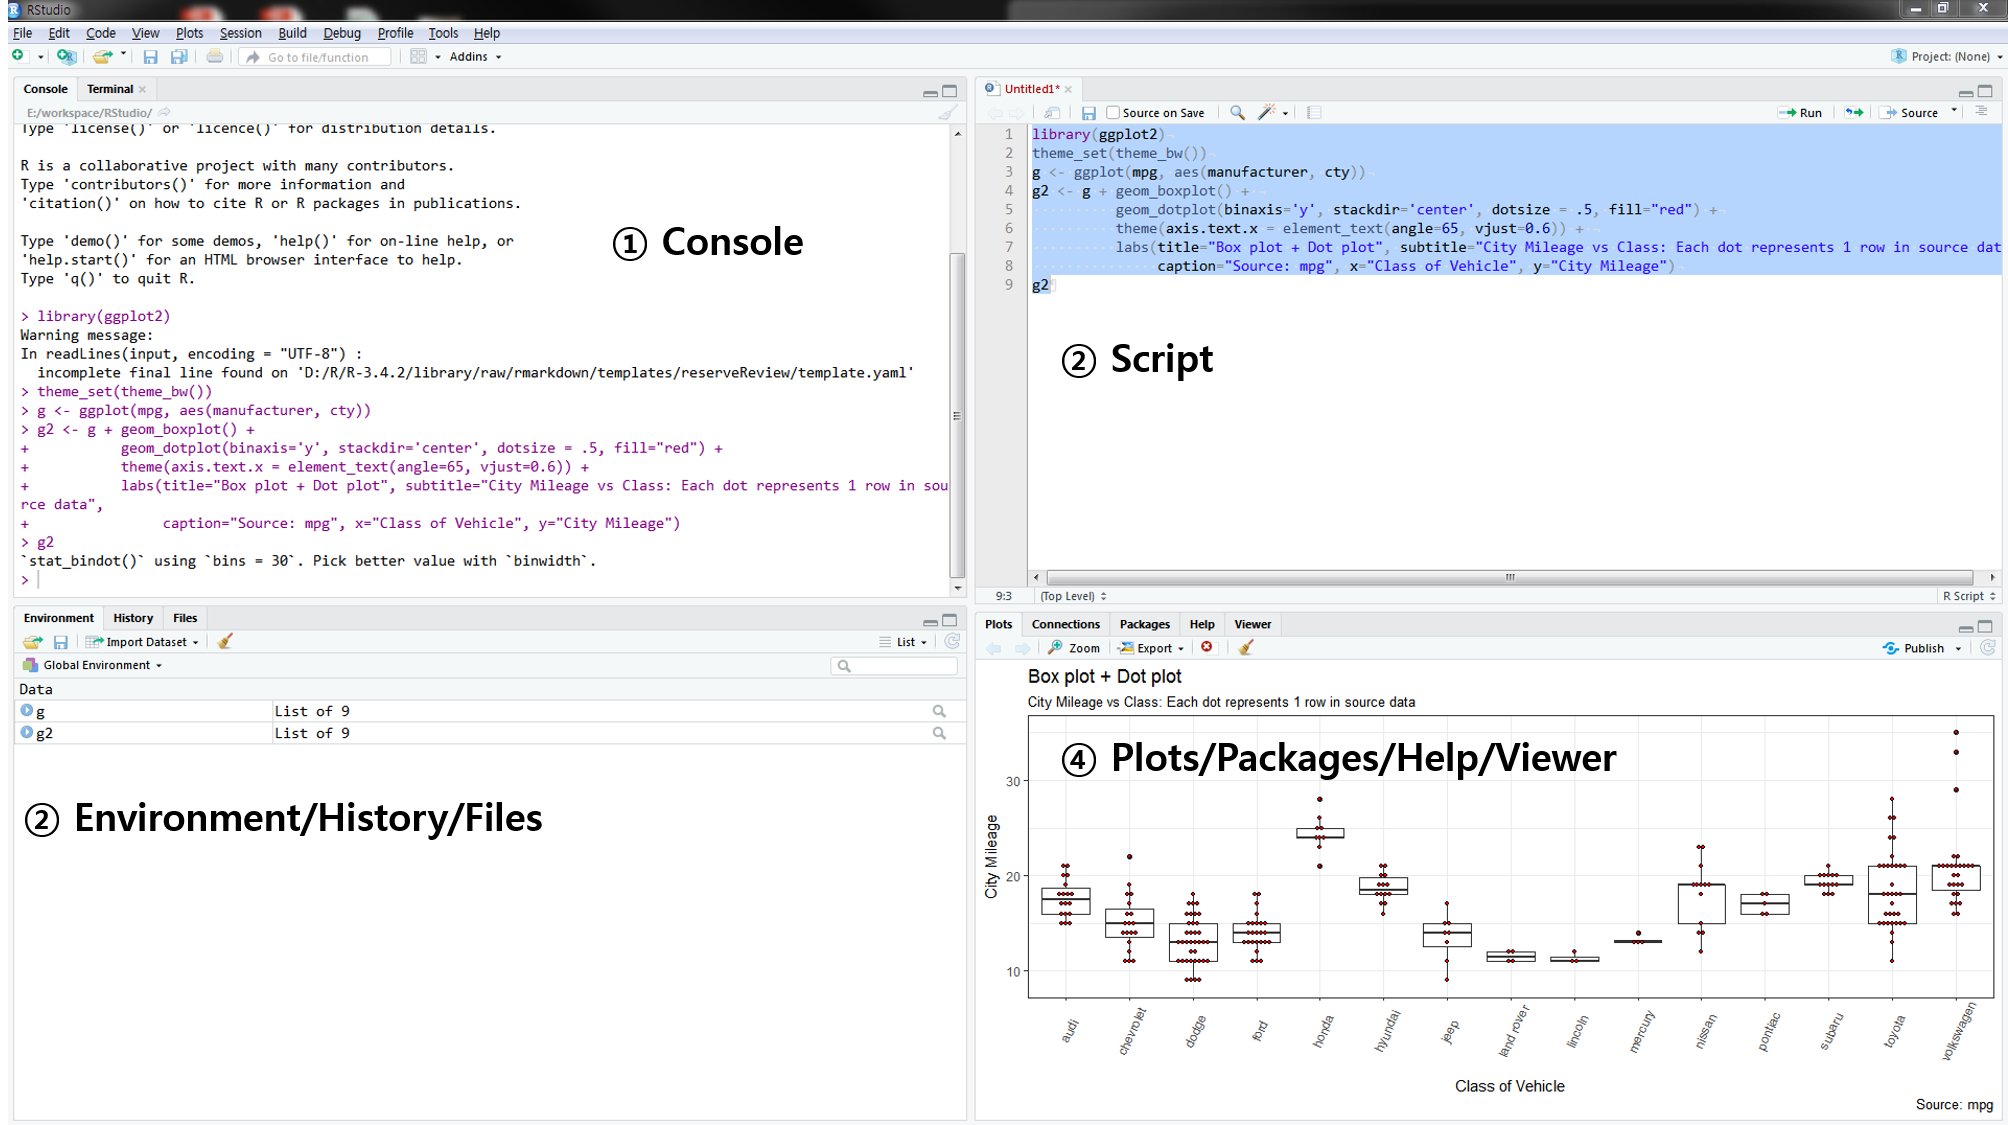
\includegraphics[width = 14cm, height = 12cm]{Figures/Rstudio-cap1.png}
        \caption[RStudio 화면구성]{RStudio 화면구성}\label{fig:Rstudio-part-01}
      }
      \end{figure}
    \end{itemize}
  \item
    Environment/History

    \begin{itemize}
    \tightlist
    \item
      Environment: 현재 R 작업환경에 저장되어 있는 객체의 특성을 요약
      제시

      \begin{itemize}
      \tightlist
      \item
        좌측 화살표 버튼 클릭: 해당 객체의 상세 정보 확인(그림
        \ref{fig:Rstudio-envirn-01})
      \item
        우측 사각형 버튼 클릭: 스프레드 시트 형태로 데이터셋 확인(그림
        \ref{fig:Rstudio-envirn-02})

        \begin{figure}[H] {
          \centering
          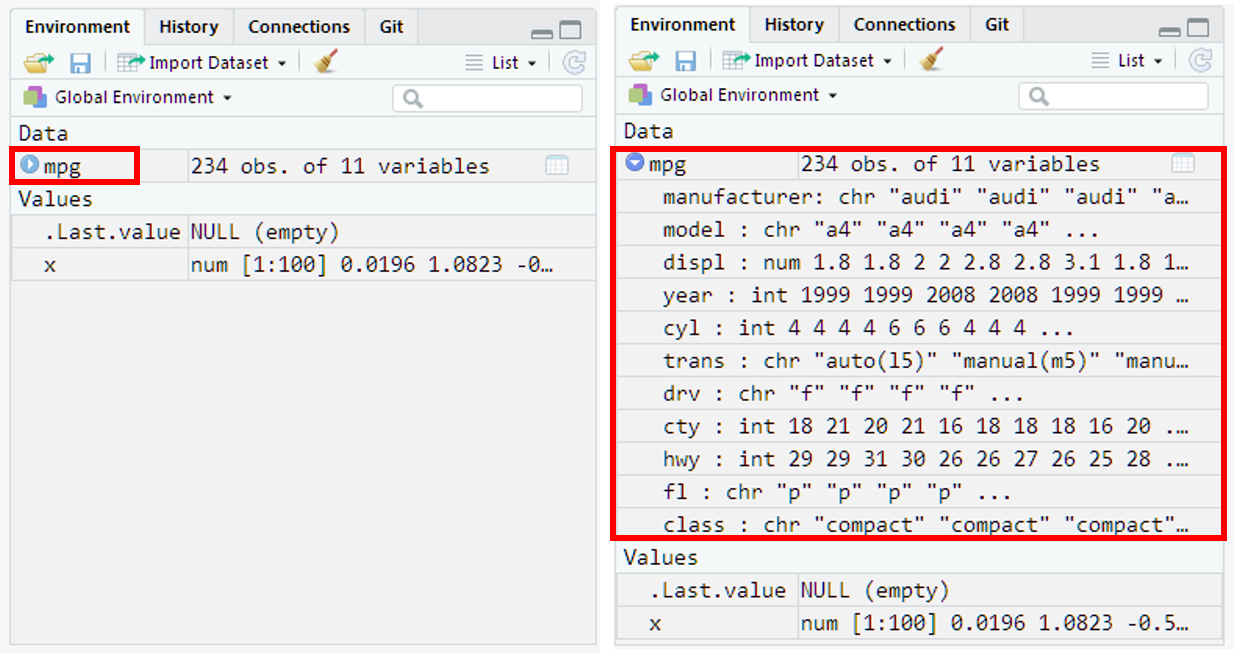
\includegraphics[width = 12cm, height = 10cm]{Figures/Rstudio-envwin-01.png}
          \caption[RStudio Environment 창: 객체 상세정보]{RStudio Environment 창: 객체 상세정보}\label{fig:Rstudio-envirn-01}
        } \end{figure}\begin{figure}[H] {
          \centering
          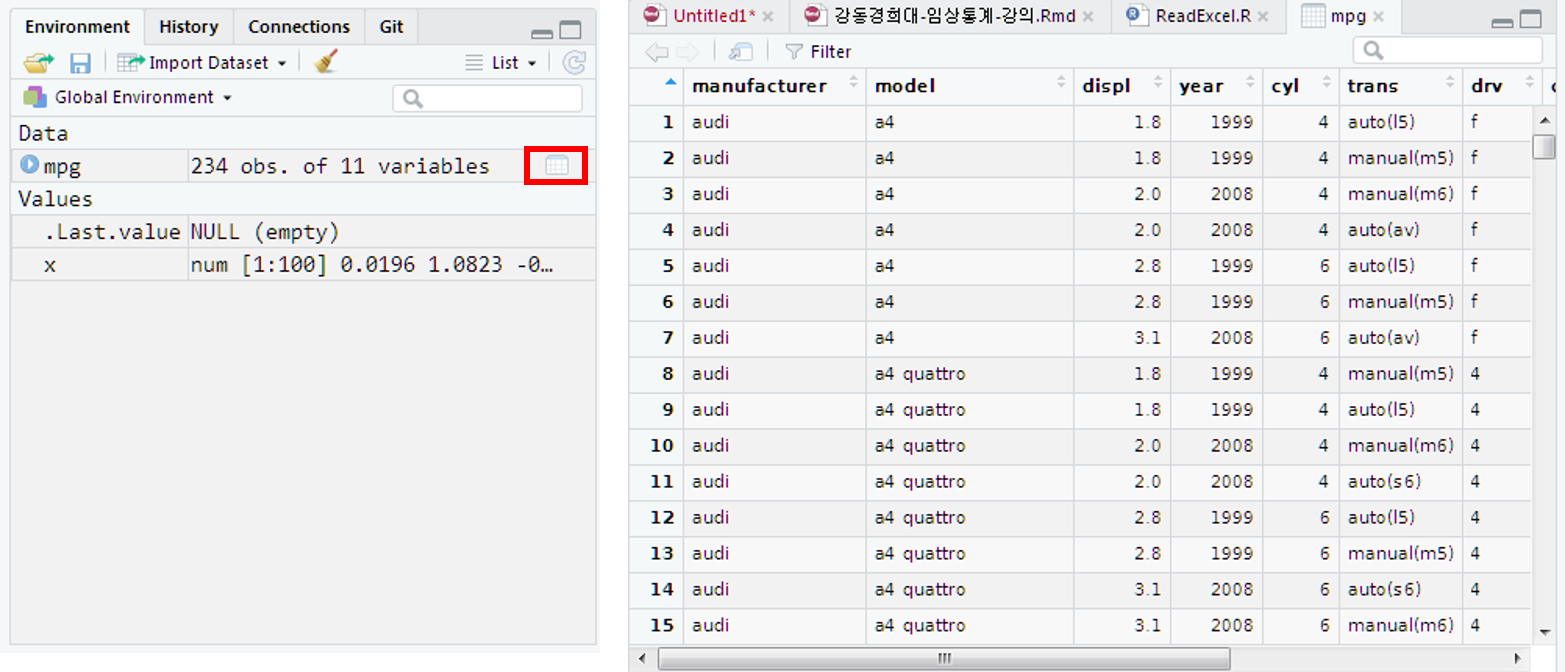
\includegraphics[width = 15cm, height = 10cm]{Figures/Rstudio-envwin-02.png}
          \caption[RStudio Environment 창: 스프레드 시트]{RStudio Environment 창: 스프레드 시트}\label{fig:Rstudio-envirn-02}
        } \end{figure}
      \end{itemize}
    \item
      History: R 콘솔에서 실행된 명령어(스크립트)들의 이력 확인

      \begin{figure}[H] {
        \centering
        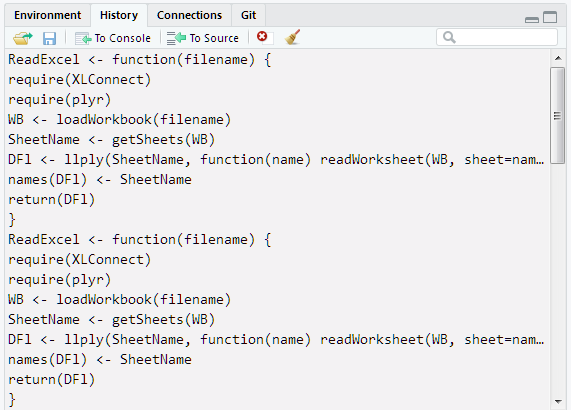
\includegraphics[width = 8cm, height = 8cm]{Figures/Rstudio-historywin.png}
        \caption[RStudio History 창]{RStudio History 창}\label{fig:Rstudio-history}
      } \end{figure}
    \end{itemize}
  \end{enumerate}
\item
  창 순서는 사용자의 편의에 따라 변경 가능

  \begin{itemize}
  \tightlist
  \item
    상단 메뉴바에서 \keystroke{Tools} \(\rightarrow\)
    \keystroke{Global Options} \(\rightarrow\)
    \keystroke{Pane Layout}에서 조정
  \end{itemize}
\end{enumerate}

\begin{figure}[H]
{
  \centering
  \includegraphics[width = 12cm, height = 10cm]{Figures/Rstudio-layout.png}
  \caption[RStudio Global Options: Pane layout]{RStudio Global Options에서 화면 레이아웃 조정}\label{fig:Rstudio-layout}
}
\end{figure}

\chapter{R의 기본 사용}\label{r--}

\section{변수}

\section{스칼라}

\section{벡터}

\section{리스트}

\section{행렬}

\section{배열}

\section{데이터 프레임}\label{-}

\chapter{데이터 조작}\label{-}

\section{파일 입출력}\label{-}

\chapter{\texorpdfstring{\texttt{ggplot2}를 이용한 자료
시각화}{ggplot2를 이용한 자료 시각화}}\label{ggplot2---}

\chapter{재현가능한 데이터 연동 문서 작성}\label{----}

\renewcommand\bibname{References}
\bibliography{CNUH.bib}


\end{document}
